% MRIxFields 2026, Task 3 -- showcase presentation, v0. About 15 minutes, 29 slides, a closing
% slide and 4 backup.
% Compile from inside reports/:  ~/anaconda3/envs/tex/bin/tectonic showcase_presentation_v0.tex
%
% Conventions
%  - One idea per build step: every multi-part slide reveals its parts with overlays.
%  - \ph{TBD} on every frame, bottom right: the presenter's initial. Replace per slide.
%  - Small inzva logo top right of every content frame (background template); the title and
%    closing frames carry the full logos instead.
%  - Palette and U-Net glyph are reports/slides_miccai.tex's.
%  - \placeholder marks an image still to be supplied (workshop photo, preprint page).
%
% Numbers: validation-phase SSIM/nRMSE/LPIPS are challenge leaderboard scores (same table as
% reports/architecture_report.tex). Final test-phase ranking: Synapse wiki "Final Ranking"
% (syn72060672, 1 Oct 2026). Local analyses: reports/error_spectrum_report.tex, TODO.md.
% Figures: scripts/make_showcase_qualitative.py and scripts/make_showcase_figures.py write
% reports/figures/showcase/; everything else is reused from the earlier decks.
\documentclass[t,aspectratio=169,11pt]{beamer}

\usetheme{default}
\usepackage{lmodern}
\usepackage[T1]{fontenc}
\usepackage{amsmath}
\usepackage{amssymb}
\usepackage{booktabs}
\usepackage{array}
\usepackage{colortbl}
\usepackage{graphicx}
\usepackage{tikz}
\usetikzlibrary{positioning,arrows.meta,fit,calc}
\usepackage{qrcode}
% backup frames count from 1 on their own; the main part's total excludes them
\usepackage{appendixnumberbeamer}

\setbeamertemplate{navigation symbols}{}
\setbeamercolor{frametitle}{fg=black}
\setbeamercolor{structure}{fg=black!70}
\setbeamerfont{frametitle}{size=\large,series=\bfseries}
\setbeamertemplate{itemize item}{\textbf{--}}

% Frame number bottom right, kept clear of the presenter initial in the corner.
\setbeamerfont{footline}{size=\scriptsize}
\setbeamercolor{footline}{fg=gray}
\setbeamertemplate{footline}{%
  \leavevmode\hfill\usebeamerfont{footline}\usebeamercolor[fg]{footline}%
  \insertframenumber\,/\,\inserttotalframenumber\hspace*{12mm}\vskip1.6mm}

% Small inzva logo, top right of every frame that does not reset the background.
\setbeamertemplate{background}{%
  \begin{tikzpicture}[remember picture, overlay]
    \node[anchor=north east, inner sep=0] at ([xshift=-4mm, yshift=-3.2mm]current page.north east)
      {\IfFileExists{logos/inzva_logo_dark.png}{
\includegraphics[height=3.2mm]{logos/inzva_logo_dark.png}}{}};
  \end{tikzpicture}}

\definecolor{base}{HTML}{9FB3C8}
\definecolor{accentfill}{HTML}{FBE4E4}
\definecolor{accent}{HTML}{D64545}
\definecolor{cond}{HTML}{3E7CB1}
\definecolor{ink}{HTML}{102A43}
\definecolor{muted}{HTML}{627D98}
\definecolor{baseline}{HTML}{D9E2EC}

\newcommand{\hl}[1]{\textcolor{accent}{\textbf{#1}}}
\newcommand{\info}[1]{\textcolor{cond}{\textbf{#1}}}
\newcommand{\gloss}[1]{{\footnotesize\textcolor{black!65}{#1}}\par}
\newcommand{\srcline}[1]{\vfill{\scriptsize\textcolor{gray}{#1}}}
\newcommand{\parttag}[1]{{\scriptsize\textcolor{muted}{#1}}\par\vspace{0.4mm}}

% Presenter initial, bottom right corner, on the frame number's baseline.
\newcommand{\ph}[1]{%
  \begin{tikzpicture}[remember picture, overlay]
    \node[anchor=base east, font=\scriptsize\bfseries, text=muted, inner sep=0pt]
      at ([xshift=-4mm, yshift=1.7mm]current page.south east) {#1};
  \end{tikzpicture}}

% An image still to be supplied: a dashed outline of the given size with its description.
\newcommand{\placeholder}[3]{%
  \begin{tikzpicture}
    \draw[draw=muted, dashed, line width=0.6pt] (0,0) rectangle (#1,#2);
    \node[align=center, text=muted, font=\footnotesize, text width=#1-6mm]
      at (#1/2,#2/2) {#3};
  \end{tikzpicture}}

% A multi-panel figure whose later panels are dimmed until their step. #1 width, #2 file,
% #3 the tikz mask commands (in figure-fraction coordinates, 0..1 both ways).
\newcommand{\maskedfigure}[3]{%
  \begin{tikzpicture}
    \node[inner sep=0, anchor=south west] (img) at (0,0) {\includegraphics[width=#1]{#2}};
    \begin{scope}[x={(img.south east)}, y={(img.north west)}]
      #3
    \end{scope}
  \end{tikzpicture}}
\tikzset{dim/.style={fill=white, opacity=0.9}}

\newcommand{\logoslot}[3]{%
  \IfFileExists{logos/#1.pdf}{\includegraphics[height=#3]{logos/#1.pdf}}{%
  \IfFileExists{logos/#1.png}{\includegraphics[height=#3]{logos/#1.png}}{%
    \raisebox{0.15\height}{\fbox{\rule{0pt}{#3}\,\textsf{\textbf{#2}}\,}}}}}

% ------------------------------------------------------------------ U-Net glyph
% Same skeleton as reports/slides_miccai.tex; red marks only what a panel changed.
\newif\ifshowin  \showintrue
\newif\ifshowout \showouttrue
\tikzset{
  blk/.style   = {draw=base, fill=baseline, rounded corners=0.4pt,
                  minimum height=2.4mm, inner sep=0pt, line width=0.3pt},
  hot/.style   = {draw=accent, fill=accentfill, line width=0.7pt},
  io/.style    = {font=\scriptsize, text=muted, inner sep=1pt},
  skip/.style  = {->, draw=base, line width=0.3pt, >={Stealth[length=1mm]}},
  flow/.style  = {->, draw=muted, line width=0.35pt, >={Stealth[length=1.2mm]}},
}
\newcommand{\unet}[1]{%
\begin{tikzpicture}[x=1mm,y=1mm,baseline]
  \path (-12,9) rectangle (25,-22);
  \foreach \i/\w in {0/9,1/7,2/5,3/3.5}{
    \node[blk,minimum width=\w mm] (e\i) at ({\i*1.7},{-\i*4}) {};
    \node[blk,minimum width=\w mm] (d\i) at ({16-\i*1.7},{-\i*4}) {};}
  \node[blk,minimum width=3mm] (b) at (8,-16.5) {};
  \foreach \i in {0,1,2,3}{ \draw[skip] (e\i) -- (d\i); }
  \foreach \i [evaluate=\i as \j using int(\i+1)] in {0,1,2}{
    \draw[flow] (e\i) -- (e\j);  \draw[flow] (d\j) -- (d\i);}
  \draw[flow] (e3) -- (b);  \draw[flow] (b) -- (d3);
  \ifshowin  \node[io,left=1.2mm of e0] (in) {$x$};  \draw[flow] (in) -- (e0);  \fi
  \ifshowout \node[io,right=1.2mm of d0] (out) {$\hat{y}$}; \draw[flow] (d0) -- (out); \fi
  #1
\end{tikzpicture}}
\newcommand{\condtokens}[1][cond]{%
  \node[draw=#1, fill=white, rounded corners=0.4pt, minimum width=7mm,
        minimum height=2.2mm, line width=0.5pt, font=\scriptsize, text=#1,
        inner sep=0.5pt] (c) at (8,-20) {$E_s\!+\!E_t$};
  \draw[->, draw=#1, line width=0.5pt, >={Stealth[length=1mm]}] (c) -- (b);}
\newcommand{\instack}[1]{%
  \foreach \k in {0,1,2,3}{
    \node[blk,hot,minimum width=2.4mm,minimum height=1.6mm] (v\k) at (-8.6,{2.8-\k*2.6}) {};}
  #1
  \draw[->,draw=accent,line width=0.4pt,>={Stealth[length=1mm]}] (-7.3,0) -- (-4.7,0);}
\newcommand{\unetpanel}[3]{%
  \begin{minipage}[t]{0.27\textwidth}\centering
    \scalebox{0.86}{\unet{#1}}\\[0.5mm]
    {\scriptsize\bfseries #2}\\[-0.3mm]
    {\scriptsize\textcolor{muted}{#3}}
  \end{minipage}}
\newcommand{\pipestage}[2]{%
  \begin{minipage}[t]{0.21\textwidth}\centering
    \parbox[c][27mm][c]{\linewidth}{\centering #1}\\[1.5mm]
    {\scriptsize #2}
  \end{minipage}}
\newcommand{\pipearrow}{%
  \begin{minipage}[t]{0.045\textwidth}\centering
    \parbox[c][27mm][c]{\linewidth}{\centering\large\textcolor{muted}{$\rightarrow$}}
  \end{minipage}}
\newcommand{\archarrow}[3]{%
  \begin{minipage}[t]{0.06\textwidth}\centering
    \vspace{8.5mm}
    {\tiny\textcolor{#2}{#3}}\\[-1.2mm]
    {\large\textcolor{muted}{$#1$}}
  \end{minipage}}

% The final-ranking table, top 9 ordered by SSIM; #1 is our row's colour command, #2 styles
% our SSIM cells. Versions are swapped with \only, since \rowcolor takes no overlay spec.
\newcommand{\finaltable}[2]{%
  {\footnotesize\setlength{\tabcolsep}{5pt}
  \begin{tabular}{lrrrrrrrr}
    \toprule
    & \multicolumn{2}{c}{SSIM $\uparrow$} & \multicolumn{2}{c}{nRMSE $\downarrow$}
      & \multicolumn{2}{c}{LPIPS $\downarrow$} & mean & final \\
    \cmidrule(lr){2-3}\cmidrule(lr){4-5}\cmidrule(lr){6-7}
    team & value & rank & value & rank & value & rank & rank & place \\
    \midrule
    Watt               & 0.94684 & 1  & 0.2253 & 1  & 0.0381 & 1  & 1.00 & 1 \\
    Blue Tent          & 0.94439 & 2  & 0.2292 & 2  & 0.0453 & 4  & 2.67 & 2 \\
    MRIxFields2026-Zhu & 0.94259 & 3  & 0.2457 & 5  & 0.0613 & 18 & 8.67 & 8 \\
    #1
    \textbf{inzva mri} & #2{0.94255} & #2{4} & 0.2480 & 6 & 0.0506 & 14 & \textbf{8.00} & \textbf{6} \\
    Lzu\_LastDance     & 0.94202 & 5  & 0.2492 & 8  & 0.0398 & 2  & 5.00 & 3 \\
    croissant          & 0.94050 & 6  & 0.2367 & 3  & 0.0472 & 7  & 5.33 & 4 \\
    Newton             & 0.93914 & 8  & 0.2445 & 4  & 0.0500 & 11 & 7.67 & 5 \\
    imispllove         & 0.93902 & 9  & 0.2530 & 9  & 0.0465 & 6  & 8.00 & 6 \\
    Tryer              & 0.93485 & 14 & 0.2558 & 10 & 0.0442 & 3  & 9.00 & 9 \\
    \bottomrule
  \end{tabular}}}

% Metrics frame: the three names along the top, the one being explained in ink.
\newcommand{\metricnav}[1]{%
  {\small\ifnum#1=1 \textcolor{ink}{\textbf{nRMSE}}\else\textcolor{muted!60}{nRMSE}\fi
   \hspace{8mm}\ifnum#1=2 \textcolor{ink}{\textbf{SSIM}}\else\textcolor{muted!60}{SSIM}\fi
   \hspace{8mm}\ifnum#1=3 \textcolor{ink}{\textbf{LPIPS}}\else\textcolor{muted!60}{LPIPS}\fi\par}}
% A stack of three feature-map channels, front one last; #1 y or p, #2 node name.
\newcommand{\featstack}[2]{%
  \node[inner sep=0, draw=white, line width=0.6pt] at (0.3,0.3)
    {\includegraphics[height=1.35cm]{figures/showcase/lpips_feat_#1_3.png}};
  \node[inner sep=0, draw=white, line width=0.6pt] at (0.15,0.15)
    {\includegraphics[height=1.35cm]{figures/showcase/lpips_feat_#1_2.png}};
  \node[inner sep=0, draw=white, line width=0.6pt] (#2) at (0,0)
    {\includegraphics[height=1.35cm]{figures/showcase/lpips_feat_#1_1.png}};}

\begin{document}

% ============================================================================ OPENING
% --------------------------------------------------------------------- 1. title
{\setbeamertemplate{background}{}
\begin{frame}[plain]
  \ph{TBD}
  \vfill
  \centering
  {\Large\bfseries Cross-Field Brain MRI Translation}\\[1.5mm]
  {\large MIM and conditioning-based approaches, MRIxFields 2026 Task 3}\\[5mm]

  {\footnotesize \mbox{Berkin Deniz Kahya\textsuperscript{1,2}}\hspace{4mm}
          \mbox{Racha Badreddine\textsuperscript{1,2}}\hspace{4mm}
          \mbox{Furkan Y\"uceyal\c{c}\i n\textsuperscript{2}}\hspace{4mm}
          \mbox{Ahmet Zelka\textsuperscript{2}}\hspace{4mm}
          \mbox{\.Ilkay \"Oks\"uz\textsuperscript{1}}}\\[2mm]
  {\footnotesize\textcolor{muted}{%
    \textsuperscript{1}\.Istanbul Technical University, PIMI Lab \quad
    \textsuperscript{2}inzva}}\\[6mm]

  \logoslot{itu_logo_siyah}{\.ITU}{12mm}\hspace{16mm}%
  \raisebox{2.2mm}{\logoslot{inzva_logo_dark}{inzva}{7mm}}\\[7mm]

  \onslide<2->{{\normalsize 3rd Place Award, Task 3 \;$\cdot$\; 4th on SSIM among 25 teams}}
  \vfill
\end{frame}
}

% ---------------------------------------------------------- 2. at MICCAI 2026
\begin{frame}{MRIxFields 2026 at MICCAI}
  \ph{TBD}
  \begin{columns}[c,onlytextwidth]
  \begin{column}{0.55\textwidth}
    \centering
    % workshop photo goes here: \includegraphics[width=\linewidth]{figures/showcase/workshop_photo.jpg}
    \placeholder{7.6cm}{5.4cm}{workshop photo\\(to be added)}
  \end{column}
  \begin{column}{0.42\textwidth}
    \begin{itemize}\setlength{\itemsep}{4mm}
      \item<1-> Presented at the MRIxFields 2026 workshop, MICCAI 2026, Strasbourg\\
            {\footnotesize\textcolor{muted}{1 October 2026, oral session}}
      \item<2-> 3rd Place Award, Task 3\\
            {\footnotesize\textcolor{muted}{top 9 of 25 teams}}
      \item<3-> 4th on SSIM\\
            6th by mean rank over SSIM, nRMSE, LPIPS
    \end{itemize}
  \end{column}
  \end{columns}
\end{frame}

% ============================================================================ I. PROBLEM
% ------------------------------------------------------------------ 3. the data
\begin{frame}{The task}
  \ph{TBD}
  \parttag{I \quad PROBLEM}
  \centering
  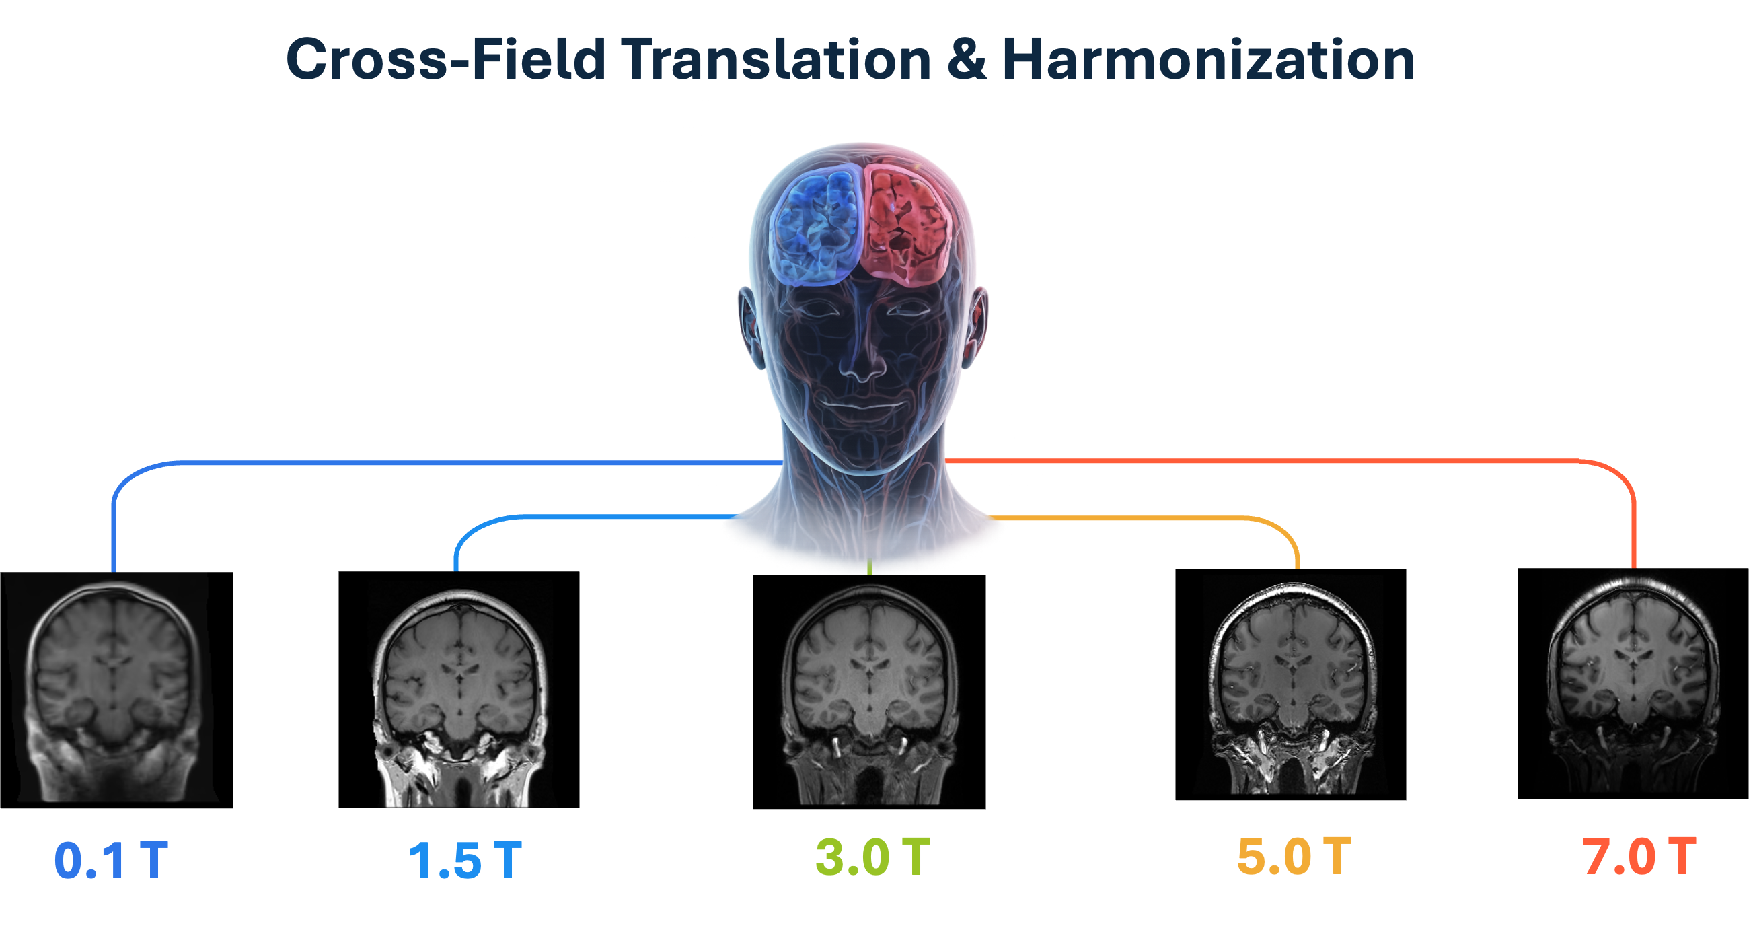
\includegraphics[height=0.62\textheight]{figures/slide_task_fields.pdf}

  \vspace{1.5mm}
  {\large Given the scan at one field strength, predict the same subject at another.}

  \vspace{0.5mm}
  \gloss{One subject, one slice. 5 field strengths $\times$ 3 contrasts (T1W, T2W, T2FLAIR),
  co-registered on one grid.}
\end{frame}

% ----------------------------------------------------------------- 4. three tasks
\begin{frame}{Tasks}
  \ph{TBD}
  \parttag{I \quad PROBLEM}
  \centering
  \vspace{2mm}
  \resizebox{0.92\linewidth}{!}{%
  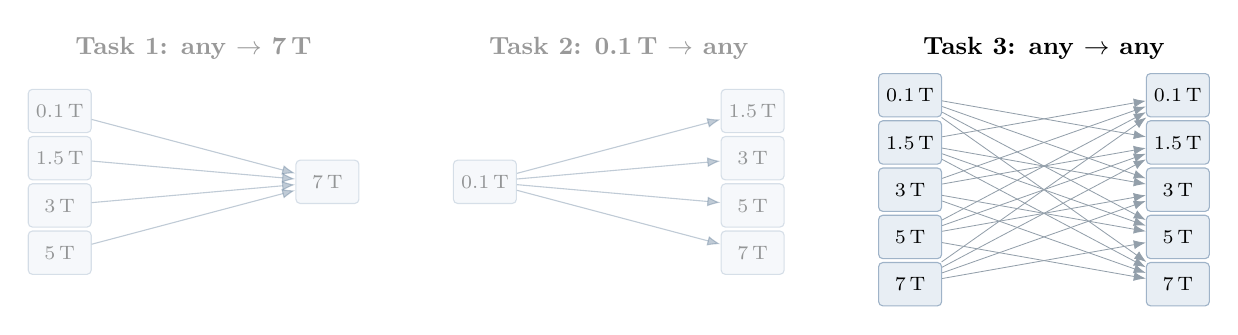
\begin{tikzpicture}[font=\scriptsize, >=Latex,
    f/.style={draw=base, fill=baseline!60, rounded corners=1.5pt, minimum width=8mm,
              minimum height=5.5mm, inner sep=1pt}]
    \begin{scope}[opacity=0.4]
      \node[font=\small\bfseries] at (1.7,1.5) {Task 1: any $\to$ 7\,T};
      \foreach \i/\y/\lab in {1/0.7/{0.1}, 2/0.1/{1.5}, 3/-0.5/{3}, 4/-1.1/{5}}
        \node[f] (a\i) at (0,\y) {\lab\,T};
      \node[f] (atgt) at (3.4,-0.2) {7\,T};
      \foreach \i in {1,...,4} \draw[->, muted] (a\i) -- (atgt);
    \end{scope}
    \begin{scope}[shift={(5.4,0)}, opacity=0.4]
      \node[font=\small\bfseries] at (1.7,1.5) {Task 2: 0.1\,T $\to$ any};
      \node[f] (bsrc) at (0,-0.2) {0.1\,T};
      \foreach \i/\y/\lab in {1/0.7/{1.5}, 2/0.1/{3}, 3/-0.5/{5}, 4/-1.1/{7}}
        \node[f] (b\i) at (3.4,\y) {\lab\,T};
      \foreach \i in {1,...,4} \draw[->, muted] (bsrc) -- (b\i);
    \end{scope}
    \begin{scope}[shift={(10.8,0)}]
      \node[font=\small\bfseries] at (1.7,1.5) {Task 3: any $\to$ any};
      \foreach \i/\y/\lab in {1/0.9/{0.1}, 2/0.3/{1.5}, 3/-0.3/{3}, 4/-0.9/{5}, 5/-1.5/{7}}{
        \node[f] (c\i) at (0,\y) {\lab\,T};
        \node[f] (d\i) at (3.4,\y) {\lab\,T};}
      \foreach \src in {1,...,5}{
        \foreach \tgt in {1,...,5}{
          \ifnum\src=\tgt\relax\else
            \draw[->, ink!45, line width=0.3pt] (c\src) -- (d\tgt);
          \fi}}
    \end{scope}
  \end{tikzpicture}}

  \vspace{6mm}
  \begin{itemize}\setlength{\itemsep}{2mm}
    \item<2-> We work on Task 3: one model for all 20 ordered field pairs $\times$ 3 contrasts,
          60 translations per subject.
    \item<3-> Metrics: SSIM (main), nRMSE, LPIPS. Final rank: mean of the three ranks.
  \end{itemize}
\end{frame}

% ------------------------------------------------------------------ 5. metrics
\begin{frame}{Metrics}
  \ph{TBD}
  \parttag{I \quad PROBLEM}
  \centering
  \only<1>{\metricnav{1}}\only<2-5>{\metricnav{2}}\only<6-8>{\metricnav{3}}
  \vspace{2mm}

  % nRMSE: the formula alone
  \only<1>{%
    \vspace{14mm}
    {\Large $\displaystyle \mathrm{nRMSE}(\hat y, y) = \frac{\lVert \hat y - y \rVert_2}{\lVert y \rVert_2}$}\par
    \vspace{10mm}
    \gloss{Pixel error, relative to the size of the target, over the brain. Lower is better.}}%
  % SSIM: three factors, then the same nRMSE at three SSIMs
  \only<2-5>{%
    {\small $\displaystyle \mathrm{SSIM}(\hat y, y) =
      \underbrace{\frac{2\mu_{\hat y}\mu_y + C_1}{\mu_{\hat y}^2 + \mu_y^2 + C_1}}_{\text{luminance}}
      \cdot
      \underbrace{\frac{2\sigma_{\hat y}\sigma_y + C_2}{\sigma_{\hat y}^2 + \sigma_y^2 + C_2}}_{\text{contrast}}
      \cdot
      \underbrace{\frac{\sigma_{\hat y y} + C_3}{\sigma_{\hat y}\sigma_y + C_3}}_{\text{structure}}$}\par
    \vspace{0.5mm}
    {\scriptsize\textcolor{muted}{mean over every 7$\times$7 window and every slice; higher is better}}\par
    \vspace{1.5mm}
    \only<2>{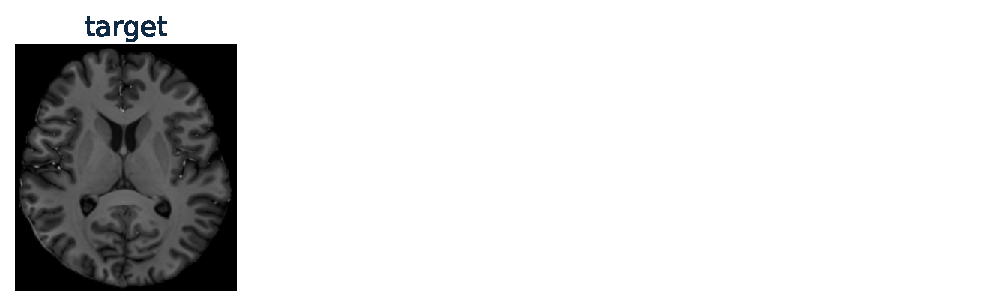
\includegraphics[width=0.70\textwidth]{figures/showcase/metric_ssim_1.pdf}}%
    \only<3>{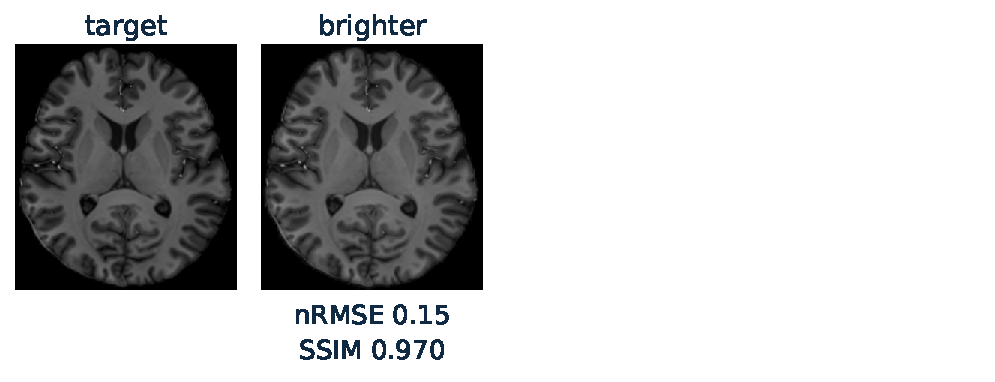
\includegraphics[width=0.70\textwidth]{figures/showcase/metric_ssim_2.pdf}}%
    \only<4>{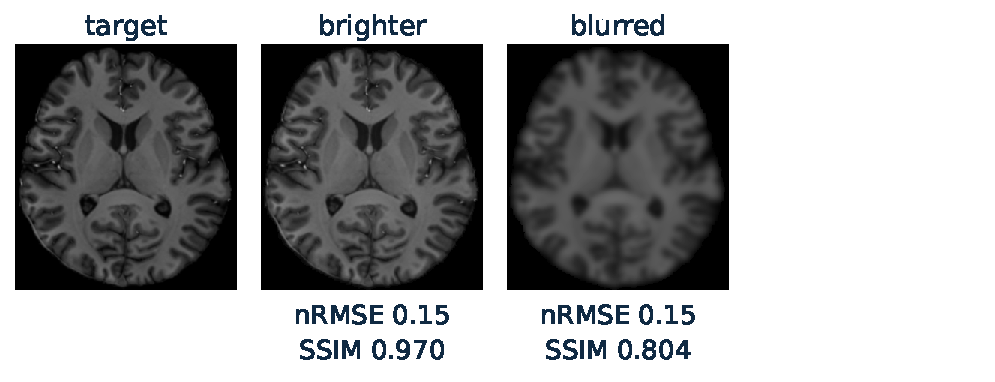
\includegraphics[width=0.70\textwidth]{figures/showcase/metric_ssim_3.pdf}}%
    \only<5>{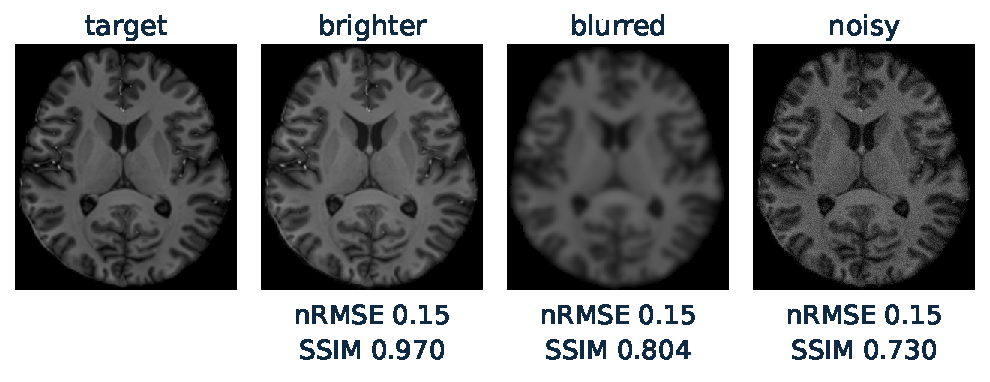
\includegraphics[width=0.70\textwidth]{figures/showcase/metric_ssim_4.pdf}}\par
    \vspace{0.5mm}
    \only<2-4>{\gloss{Each distortion has the same pixel error: nRMSE 0.15.}}%
    \only<5>{\gloss{Same nRMSE, three SSIMs: SSIM scores local structure, not pixel error.}}}%
  % LPIPS: the same encoder on both images, distance between activations
  \only<6-8>{%
    \vspace{1mm}
    \begin{tikzpicture}[font=\scriptsize, >={Stealth[length=1.4mm]}]
      \node[inner sep=0] (y) at (0,1.1)
        {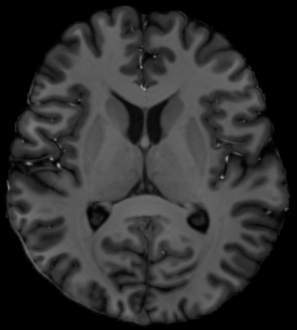
\includegraphics[height=1.6cm]{figures/showcase/lpips_target.png}};
      \node[inner sep=0] (p) at (0,-1.1)
        {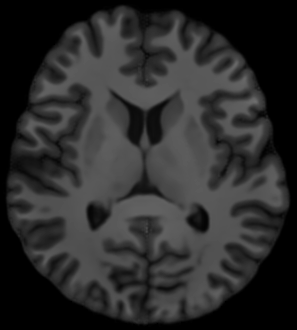
\includegraphics[height=1.6cm]{figures/showcase/lpips_pred.png}};
      \node[left=1.5mm of y, text=ink, align=right] {target\\$y$};
      \node[left=1.5mm of p, text=ink, align=right] {prediction\\$\hat y$};
      \foreach \yy in {1.1,-1.1}{
        \draw[draw=base, fill=baseline!60, line width=0.5pt]
          (1.4,\yy+0.58) -- (2.6,\yy+0.29) -- (2.6,\yy-0.29) -- (1.4,\yy-0.58) -- cycle;
        \node[text=ink] at (2.0,\yy) {AlexNet};
        \draw[->, draw=muted, line width=0.5pt] (0.8,\yy) -- (1.4,\yy);
        \draw[->, draw=muted, line width=0.5pt] (2.6,\yy) -- (3.1,\yy);}
      \node[text=muted] at (2.0,0) {same weights};
      \begin{scope}[shift={(3.75,0.95)}] \featstack{y}{fy} \end{scope}
      \begin{scope}[shift={(3.75,-1.25)}] \featstack{p}{fp} \end{scope}
      \node[text=ink, anchor=west] (ly) at (4.75,0.95) {$\hat\phi_l(y)$};
      \node[text=ink, anchor=west] (lp) at (4.75,-1.25) {$\hat\phi_l(\hat y)$};
      \node[text=muted] at (3.95,-2.3) {layer 1 of 5, 3 of 64 channels};
      \onslide<7->{%
        \node[text=ink] (diff) at (7.35,0)
          {$\lVert w_l \odot (\hat\phi_l(y) - \hat\phi_l(\hat y)) \rVert_2^2$};
        \draw[->, draw=muted, line width=0.5pt] (ly.east) to[out=0, in=110] (diff.north);
        \draw[->, draw=muted, line width=0.5pt] (lp.east) to[out=0, in=-110] (diff.south);
        \node[inner sep=0] (d) at (10.0,0)
          {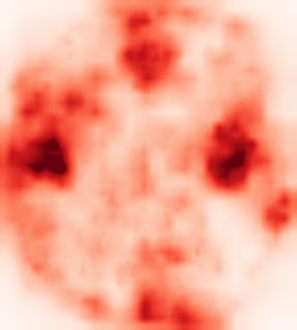
\includegraphics[height=1.6cm]{figures/showcase/lpips_dist.png}};
        \draw[->, draw=muted, line width=0.5pt] (diff.east) -- (d.west);
        \node[text=ink, align=center, above=1mm of d] {distance map,\\summed over 5 layers};}
      \onslide<8->{%
        \node[text=ink, align=center, below=1mm of d] {mean: LPIPS \textbf{0.125}};}
    \end{tikzpicture}\par
    \vspace{2mm}
    \only<6>{\gloss{Target and our prediction (0.1\,T $\to$ 7\,T, T1W, one slice) go through the
      same pretrained encoder.}}%
    \only<7>{\gloss{At each position, the squared difference of the unit-length activations,
      weighted per channel. Darker red: larger distance.}}%
    \only<8>{{\small $\displaystyle \mathrm{LPIPS}(\hat y, y) = \sum_{l=1}^{5} \frac{1}{H_l W_l}
      \sum_{h,w} \lVert w_l \odot (\hat\phi_l^{hw}(y) - \hat\phi_l^{hw}(\hat y)) \rVert_2^2$}\par
      \vspace{0.5mm}
      \gloss{An RMSE-like distance between activations, not pixels. Lower is better.}}}
\end{frame}

% ------------------------------------------------------------------ 6. data
\begin{frame}{Data}
  \ph{TBD}
  \parttag{I \quad PROBLEM}
  \centering
  \vspace{4mm}
  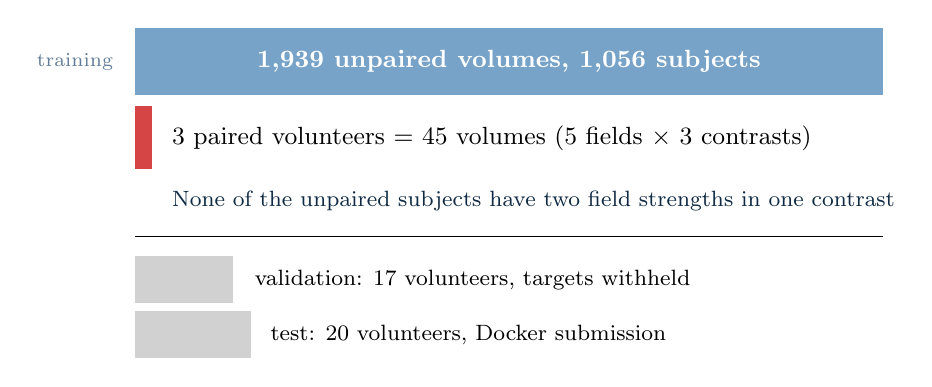
\begin{tikzpicture}[font=\small]
    % bar widths share one scale: 9.5 cm = 1,939 volumes
    \fill[cond!70] (0,0) rectangle (9.5,0.85);
    \node[white, font=\small\bfseries] at (4.75,0.42) {1{,}939 unpaired volumes, 1{,}056 subjects};
    \node[left, font=\scriptsize, text=muted] at (-0.15,0.42) {training};
    \onslide<2->{
      \fill[accent] (0,-0.95) rectangle (0.22,-0.15);
      \node[right] at (0.35,-0.55) {3 paired volunteers = 45 volumes (5 fields $\times$ 3 contrasts)};}
    \onslide<3->{
      \node[right, text=ink, font=\footnotesize] at (0.35,-1.35)
        {None of the unpaired subjects have two field strengths in one contrast};}
    \onslide<4->{
      \draw[baseline] (0,-1.8) -- (9.5,-1.8);
      \fill[black!18] (0,-2.65) rectangle (1.25,-2.05);
      \node[right, font=\footnotesize] at (1.4,-2.35) {validation: 17 volunteers, targets withheld};
      \fill[black!18] (0,-3.35) rectangle (1.47,-2.75);
      \node[right, font=\footnotesize] at (1.6,-3.05) {test: 20 volunteers, Docker submission};}
  \end{tikzpicture}
\end{frame}

% ------------------------------------------------------------------ 7. baseline
\begin{frame}{Baseline: copy the input}
  \ph{TBD}
  \parttag{I \quad PROBLEM}
  {\footnotesize Source and target share the anatomy, so copying the input already scores.}

  \vspace{1mm}
  \begin{columns}[c,onlytextwidth]
  \begin{column}{0.46\textwidth}
    \centering
    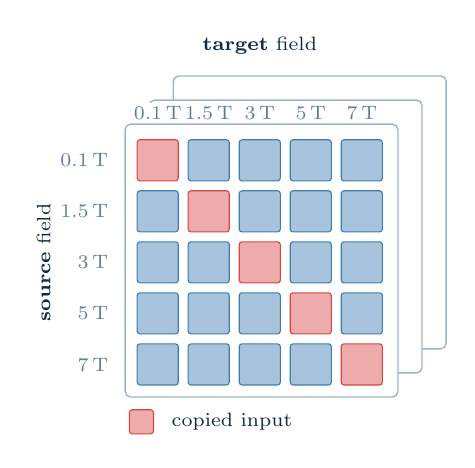
\begin{tikzpicture}[x=0.9cm,y=0.9cm,font=\scriptsize]
      \foreach \o in {2,1}{
        \draw[draw=base,fill=white,line width=0.5pt,rounded corners=2pt]
          ({-0.10+0.34*\o},{-3.70+0.34*\o}) rectangle ++(3.85,3.85);}
      \draw[draw=base,fill=white,line width=0.5pt,rounded corners=2pt]
        (-0.10,-3.70) rectangle ++(3.85,3.85);
      \foreach \c/\f in {0/0.1,1/1.5,2/3,3/5,4/7}{
        \node[text=muted,fill=white,inner sep=1.2pt] at ({\c*0.72+0.36},0.31) {\f\,T};
        \node[text=muted,anchor=east] at (-0.20,{-\c*0.72-0.36}) {\f\,T};}
      \node[text=ink] at (1.80,1.26) {\textbf{target} field};
      \node[text=ink,rotate=90] at (-1.25,-1.80) {\textbf{source} field};
      \foreach \r in {0,1,2,3,4}{
        \foreach \c in {0,1,2,3,4}{
          \ifnum\r=\c
            \fill[accent!45,draw=accent,line width=0.4pt,rounded corners=1pt]
              ({\c*0.72+0.07},{-\r*0.72-0.07}) rectangle ++(0.58,-0.58);
          \else
            \fill[cond!45,draw=cond,line width=0.4pt,rounded corners=1pt]
              ({\c*0.72+0.07},{-\r*0.72-0.07}) rectangle ++(0.58,-0.58);
          \fi}}
      \fill[accent!45,draw=accent,line width=0.4pt,rounded corners=1pt]
        (-0.04,-4.22) rectangle ++(0.34,0.34);
      \node[text=ink,anchor=west] at (0.42,-4.05) {copied input};
    \end{tikzpicture}

    \vspace{2mm}
    \gloss{All 20 ordered field pairs, in 3 contrasts.}
  \end{column}
  \begin{column}{0.5\textwidth}
    \centering
    \begin{tabular}{lcc}
      \toprule
      & SSIM & nRMSE \\
      \midrule
      \onslide<2->{$\hat y = x$ (copy)} & \onslide<2->{0.836497} & \onslide<2->{0.5216} \\
      \onslide<3->{our final model} & \onslide<3->{\textbf{0.913652}} & \onslide<3->{0.2380} \\
      \bottomrule
    \end{tabular}

    \vspace{3mm}
    \onslide<3->{\gloss{Validation phase, challenge scores.}}
  \end{column}
  \end{columns}
\end{frame}

% =================================================================== II. ANALYSES
% ------------------------------------------------------------ 8. spectral slopes
\begin{frame}{Power spectrum analysis}
  \ph{TBD}
  \parttag{II \quad ANALYSES}
  \centering
  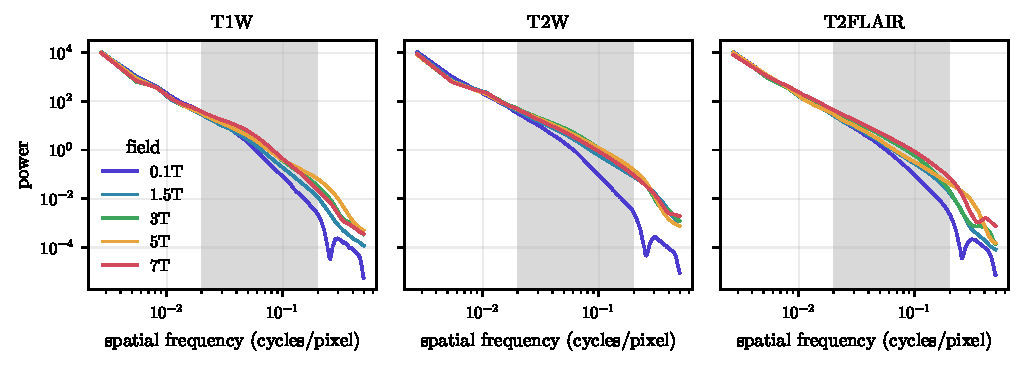
\includegraphics[width=0.80\textwidth]{spectral/fig_rapsd_by_field_retro.pdf}

  \vspace{-1mm}
  \begin{columns}[t,onlytextwidth]
  \begin{column}{0.53\textwidth}
    \onslide<2->{%
    \centering\scriptsize
    \setlength{\tabcolsep}{3.5pt}
    $P(f)\propto f^{-\alpha}$,\quad
    $\Delta\alpha=\alpha_{\text{source}}-\alpha_{7\,\mathrm{T}}$\par
    \vspace{0.6mm}
    \begin{tabular}{lcccc}
      \toprule
       & 0.1\,T & 1.5\,T & 3\,T & 5\,T \\
      \midrule
      T1W     & \hl{$+1.01$} & $+0.16$ & $-0.17$ & \info{$-0.51$} \\
      T2W     & \hl{$+1.50$} & $+0.10$ & $-0.06$ & \info{$-0.21$} \\
      T2FLAIR & \hl{$+1.29$} & $+0.35$ & $+0.34$ & $+0.18$ \\
      \bottomrule
    \end{tabular}}
  \end{column}
  \begin{column}{0.45\textwidth}
    \footnotesize
    \begin{itemize}\setlength{\itemsep}{1.2mm}
      \item<3-> 0.1\,T holds ${\sim}3\%$ of 7\,T's fine detail; the rest has to be generated.
      \item<4-> 3\,T and 5\,T are already as fine as 7\,T; the mapping is mostly contrast.
    \end{itemize}
  \end{column}
  \end{columns}

  \vspace{1mm}
  {\scriptsize\textcolor{gray}{Radially averaged power spectral density, slope fitted on
  0.02--0.2 cycles/pixel, 30 retrospective volumes per cell.}\par}
\end{frame}

% --------------------------------------------------------------- 9. error split
\begin{frame}{Error by field strength}
  \ph{TBD}
  \parttag{II \quad ANALYSES}
  \centering
  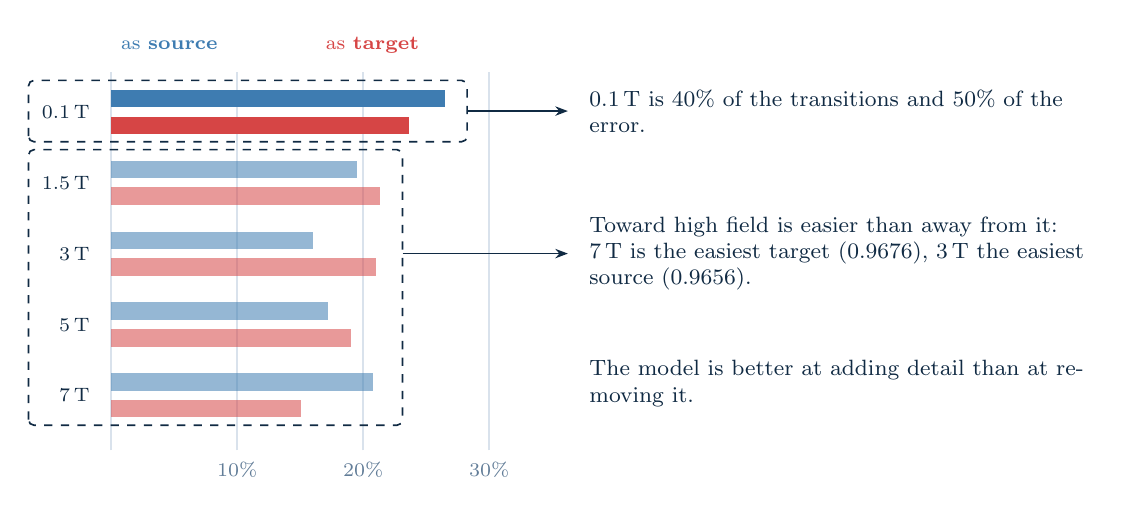
\begin{tikzpicture}[x=1cm,y=1cm,font=\scriptsize]
    \draw[draw=baseline,line width=0.8pt] (0,-0.3) -- (0,4.5);
    \foreach \x in {10,20,30}{
      \draw[draw=baseline,line width=0.6pt] (\x*0.16,-0.3) -- (\x*0.16,4.5);
      \node[text=muted] at (\x*0.16,-0.55) {\x\%};}
    \foreach \y/\lab/\s/\t/\op in {%
      4.0/0.1\,T/26.5/23.6/1.0, 3.1/1.5\,T/19.5/21.3/0.55,
      2.2/3\,T/16.0/21.0/0.55, 1.3/5\,T/17.2/19.0/0.55, 0.4/7\,T/20.8/15.1/0.55}{
      \node[anchor=east,text=ink] at (-0.15,\y) {\lab};
      \fill[cond,opacity=\op]   (0,\y+0.06) rectangle (\s*0.16,\y+0.28);
      \fill[accent,opacity=\op] (0,\y-0.28) rectangle (\t*0.16,\y-0.06);}
    \node[text=cond,anchor=west,font=\scriptsize] at (0,4.85) {as \textbf{source}};
    \node[text=accent,anchor=west,font=\scriptsize] at (2.6,4.85) {as \textbf{target}};
    \draw<1->[draw=ink,dashed,line width=0.6pt,rounded corners=2pt]
      (-1.05,3.62) rectangle (4.52,4.40);
    \draw<1->[->,draw=ink,line width=0.6pt,>={Stealth[length=1.6mm]}]
      (4.52,4.01) -- (5.80,4.01);
    \node<1->[anchor=west,text width=6.6cm,align=left,font=\footnotesize,text=ink]
      at (5.95,4.01)
      {0.1\,T is 40\% of the transitions and 50\% of the error.};
    \draw<2->[draw=ink,dashed,line width=0.6pt,rounded corners=2pt]
      (-1.05,0.02) rectangle (3.70,3.52);
    \draw<2->[->,draw=ink,line width=0.6pt,>={Stealth[length=1.6mm]}]
      (3.70,2.20) -- (5.80,2.20);
    \node<2->[anchor=west,text width=6.6cm,align=left,font=\footnotesize,text=ink]
      at (5.95,2.20)
      {Toward high field is easier than away from it: 7\,T is the easiest
       target (0.9676), 3\,T the easiest source (0.9656).};
    \node<3->[anchor=west,text width=6.6cm,align=left,font=\footnotesize,text=ink]
      at (5.95,0.55)
      {The model is better at adding detail than at removing it.};
  \end{tikzpicture}
  \srcline{Share of $\sum(1-\mathrm{SSIM})$ over 180 transitions, local scoring. Each colour
  sums to 100\%.}
\end{frame}

% ------------------------------------------------------------- 10. two regimes
\begin{frame}{Residual maps}
  \ph{TBD}
  \parttag{II \quad ANALYSES}
  \centering
  \maskedfigure{0.60\textwidth}{figures/slide_two_regimes.pdf}{%
    \fill<1>[dim] (0,0) rectangle (1.01,0.51);}

  \vspace{0.5mm}
  \only<1>{\gloss{0.1\,T $\to$ 7\,T: the residual is on the cortical folds.}}%
  \only<2>{\gloss{3\,T $\to$ 7\,T: the residual is at the outer brain edge.}}
  \gloss{Blue: too dark; red: too bright. Subject 0006, T1W.}
\end{frame}

% ------------------------------------------------------- 11. measurement limits
\begin{frame}{Measurement limits}
  \ph{TBD}
  \parttag{II \quad ANALYSES}
  \centering
  \vspace{1mm}
  {\small\renewcommand{\arraystretch}{1.35}
  \begin{tabular}{lr}
    \toprule
    Measurement & Result \\
    \midrule
    \onslide<1->{0.1\,T samples weighted $\times$1.5 in the loss}
      & \onslide<1->{$-0.0017$ local SSIM} \\
    \onslide<2->{Same method, each paired subject held out in turn}
      & \onslide<2->{0.898 to 0.920 (sd 0.011)} \\
    \onslide<3->{Same configuration, three seeds} & \onslide<3->{sd 0.0012} \\
    \onslide<4->{Checkpoint preferred by every local check, on the leaderboard}
      & \onslide<4->{$-0.00023$} \\
    \bottomrule
  \end{tabular}}

  \vspace{3mm}
  \raggedright
  \begin{itemize}\setlength{\itemsep}{2mm}
    \item<5-> The 0.1\,T error does not shrink with more loss weight: the information is not in
          the input.
    \item<6-> Differences below 0.001 were judged on the leaderboard, not locally.
  \end{itemize}
\end{frame}

% ================================================================== III. METHOD
% ---------------------------------------------------------------- 12. the model
\begin{frame}{Method}
  \ph{TBD}
  \parttag{III \quad METHOD}
  \centering
  \vspace{2mm}
  \onslide<1->{\pipestage{%
    \begin{tikzpicture}[x=1mm,y=1mm,font=\scriptsize]
      \path (-9,13) rectangle (13,-14);
      \foreach \k in {3,2,1}{
        \draw[draw=base,fill=white,line width=0.5pt,rounded corners=0.6pt]
          ({\k*1.4-7.6},{\k*1.4-8.5}) rectangle ++(15.2,17);}
      \node[inner sep=0] at (0,0)
        {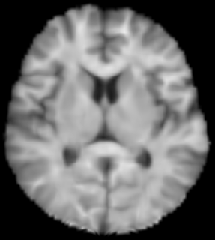
\includegraphics[height=17mm]{figures/slide_method_input.pdf}};
      \draw[draw=base,line width=0.5pt,rounded corners=0.6pt]
        (-7.6,-8.5) rectangle ++(15.2,17);
    \end{tikzpicture}}%
    {one axial slice,\\\textbf{4 co-registered channels}\\[0.4mm]
     \textcolor{muted}{the target contrast + T1W, T2W, FLAIR}}}%
  \onslide<2->{\pipearrow
  \pipestage{%
    \scalebox{0.72}{\unet{%
      \condtokens
      \node[draw=cond,fill=white,rounded corners=0.4pt,minimum width=4mm,
            minimum height=2.2mm,line width=0.5pt,font=\scriptsize,text=cond,
            inner sep=0.5pt] (z) at (18,-20) {$z$};
      \draw[->,draw=cond,line width=0.5pt,>={Stealth[length=1mm]}] (z) -- (c);}}}%
    {32-channel conditional U-Net\\\textcolor{cond}{source, target, slice $z$}\\[0.4mm]
     \textcolor{muted}{MIM-pretrained on 1{,}939 volumes}}}%
  \onslide<3->{\pipearrow
  \pipestage{%
    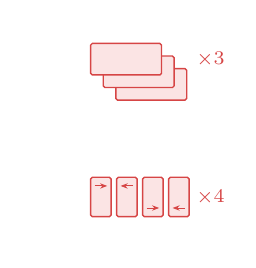
\begin{tikzpicture}[x=1mm,y=1mm,font=\scriptsize]
      \path (-8,13) rectangle (13,-14);
      \foreach \k in {2,1,0}{
        \draw[draw=accent,fill=accentfill,line width=0.5pt,rounded corners=0.6pt]
          ({\k*1.6},{7-\k*1.6}) rectangle ++(9,4);}
      \node[text=accent,anchor=west,inner sep=1pt] at (13,9) {$\times 3$};
      \foreach \k/\sx/\sy in {0/1/1,1/-1/1,2/1/-1,3/-1/-1}{
        \draw[draw=accent,fill=accentfill,line width=0.5pt,rounded corners=0.6pt]
          ({\k*3.3},-6) rectangle ++(2.6,-5);
        \draw[->,draw=accent,line width=0.35pt,>={Stealth[length=0.9mm]}]
          ({\k*3.3+1.3-\sx*0.8},{-8.5+\sy*1.4}) -- ({\k*3.3+1.3+\sx*0.8},{-8.5+\sy*1.4});}
      \node[text=accent,anchor=west,inner sep=1pt] at (13,-8.5) {$\times 4$};
    \end{tikzpicture}}%
    {\textcolor{accent}{mean of 3 checkpoints,\\mean of 4 flipped inputs}\\[0.4mm]
     \textcolor{muted}{no training}}}%
  \onslide<4->{\pipearrow
  \pipestage{%
    \begin{tikzpicture}[x=1mm,y=1mm,font=\scriptsize]
      \path (-9,13) rectangle (13,-14);
      \foreach \k in {4,3,2,1}{
        \draw[draw=base,fill=white,line width=0.5pt,rounded corners=0.6pt]
          ({\k*1.4-7.6},{\k*1.4-8.5}) rectangle ++(15.2,17);}
      \node[inner sep=0] at (0,0)
        {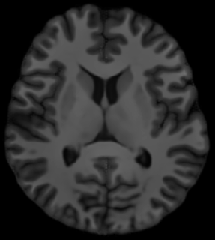
\includegraphics[height=17mm]{figures/slide_method_output.pdf}};
      \draw[draw=accent,line width=0.5pt,rounded corners=0.6pt]
        (-7.6,-8.5) rectangle ++(15.2,17);
    \end{tikzpicture}}%
    {\textcolor{accent}{prediction at the target field},\\stacked into the submitted slab}}

  \vspace{3mm}
  \onslide<2->{{\footnotesize
   conditioning $c = E_{\mathrm{src}}(d_s) + E_{\mathrm{tgt}}(d_t) + E_{z}(z)$, at the bottleneck
   and through FiLM\\[0.8mm]
   loss $L_1 + 0.5\,(1-\mathrm{SSIM}) + 0.05\,\mathrm{LPIPS}$\par}}
\end{frame}

% ------------------------------------------------------------ 13. the ladder
\begin{frame}{Ablations}
  \ph{TBD}
  \parttag{III \quad METHOD}
  \centering
  \onslide<1->{\unetpanel{}{vanilla U-Net}{0.869856}}%
  \onslide<2->{\archarrow{\rightarrow}{cond}{$+0.0278$}}%
  \onslide<2->{\unetpanel{\condtokens}{$+$ domain conditioning}{0.897646}}%
  \onslide<3->{\archarrow{\rightarrow}{accent}{$-0.0048$}}%
  \onslide<3->{\unetpanel{%
    \condtokens
    \foreach \i/\w in {0/9,1/7,2/5,3/3.5}{\node[blk,hot,minimum width=\w mm] at (d\i) {};}
    \node[draw=accent,fill=accentfill,line width=0.6pt,rounded corners=0.4pt,
          font=\scriptsize,text=accent,inner sep=1pt] at (19,-12) {$x+f(x)$};
  }{$+$ FiLM \& residual}{0.892839}}%
  \onslide<4->{\archarrow{\downarrow}{cond}{$+0.0103$}}

  \vspace{-3mm}

  {\showinfalse
  \onslide<4->{\unetpanel{%
    \condtokens
    \foreach \i/\w in {0/9,1/7,2/5,3/3.5}{
      \node[blk,hot,minimum width=\w mm] at (e\i) {};
      \node[blk,hot,minimum width=\w mm] at (d\i) {};}
    \node[blk,hot,minimum width=3mm] at (b) {};
    \foreach \r in {0,1,2}{\foreach \c in {0,1,2}{
      \fill[fill=baseline,draw=base,line width=0.2pt]
        ({-10.4+\c*1.6},{-2.4+\r*1.6}) rectangle ++(1.5,1.5);}}
    \foreach \r/\c in {0/1,1/0,1/2,2/1}{
      \fill[ink] ({-10.4+\c*1.6},{-2.4+\r*1.6}) rectangle ++(1.5,1.5);}
    \draw[->,draw=accent,line width=0.4pt,>={Stealth[length=1mm]}] (-5.7,0) -- (-4.7,0);
  }{$+$ MIM pretraining}{0.903110}}%
  \onslide<5->{\archarrow{\rightarrow}{cond}{$+0.0037$}}%
  \onslide<5->{\unetpanel{%
    \condtokens
    \node[blk,hot,minimum width=9mm] at (e0) {};
    \instack{\foreach \k/\lab in {0/{$x$},1/t1,2/t2,3/fl}{
      \node[font=\scriptsize,text=muted,inner sep=0.4pt,anchor=east] at (-10.1,{2.8-\k*2.6}) {\lab};}}
  }{$+$ multi contrast input}{0.906773}}%
  \onslide<6->{\archarrow{\rightarrow}{cond}{$+0.0069$}}%
  \onslide<6->{\unetpanel{%
    \condtokens
    \foreach \i/\w in {0/9,1/7,2/5,3/3.5}{
      \node[blk,hot,minimum width=\w mm] at (e\i) {};
      \node[blk,hot,minimum width=\w mm] at (d\i) {};}
    \node[blk,hot,minimum width=3mm] at (b) {};
    \instack{}
  }{$+$ SSIM loss, average \& flip TTA}{\textcolor{accent}{\textbf{0.913652}}}}%
  \begin{minipage}[t]{0.06\textwidth}\hfill\end{minipage}\par}
\end{frame}

% ------------------------------------------------- 14. qualitative, to a higher field
\begin{frame}{Predictions to a higher field}
  \ph{TBD}
  \parttag{III \quad METHOD}
  \centering
  \only<1>{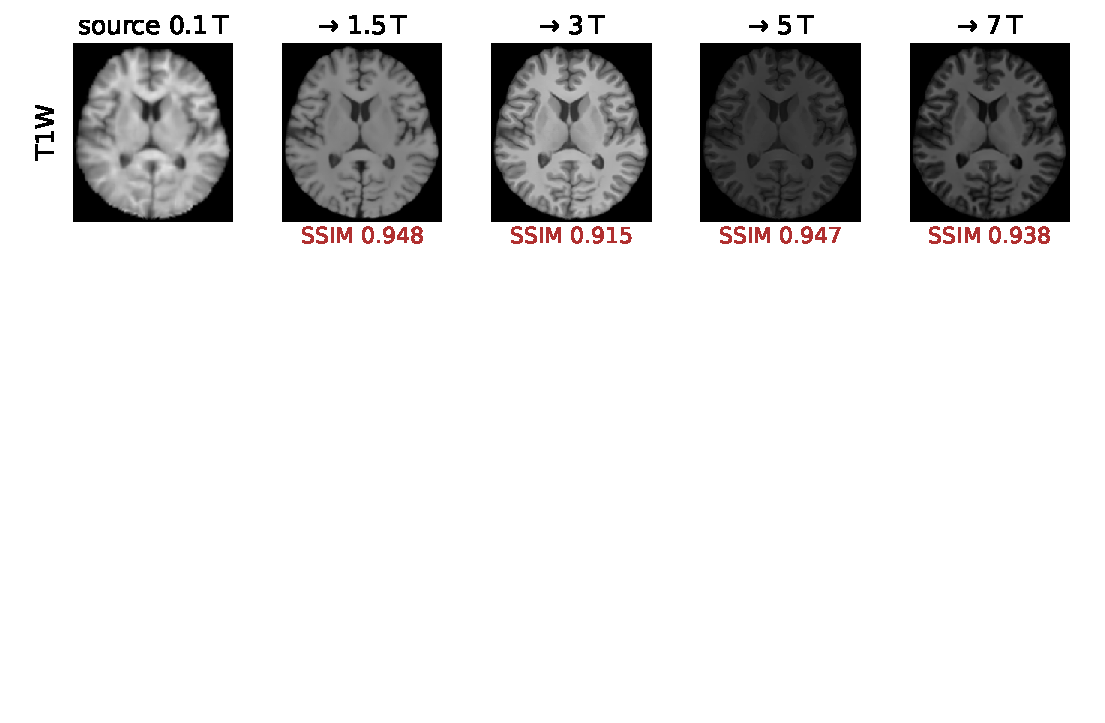
\includegraphics[height=0.76\textheight]{figures/showcase/grid_up_1.pdf}}%
  \only<2>{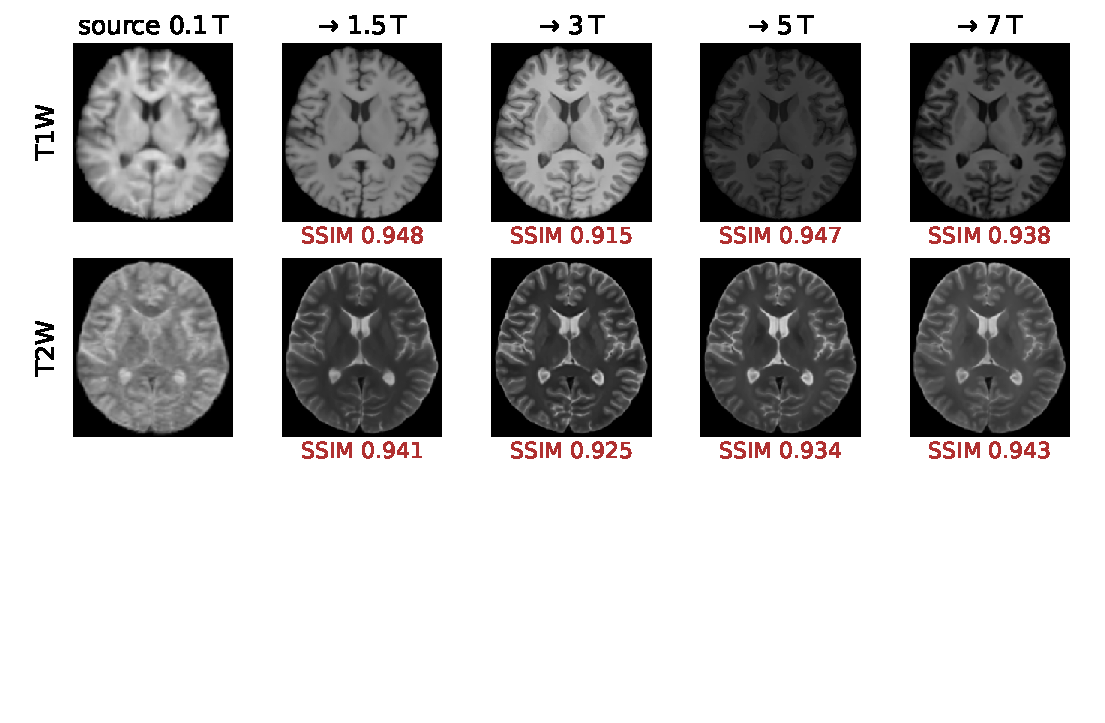
\includegraphics[height=0.76\textheight]{figures/showcase/grid_up_2.pdf}}%
  \only<3>{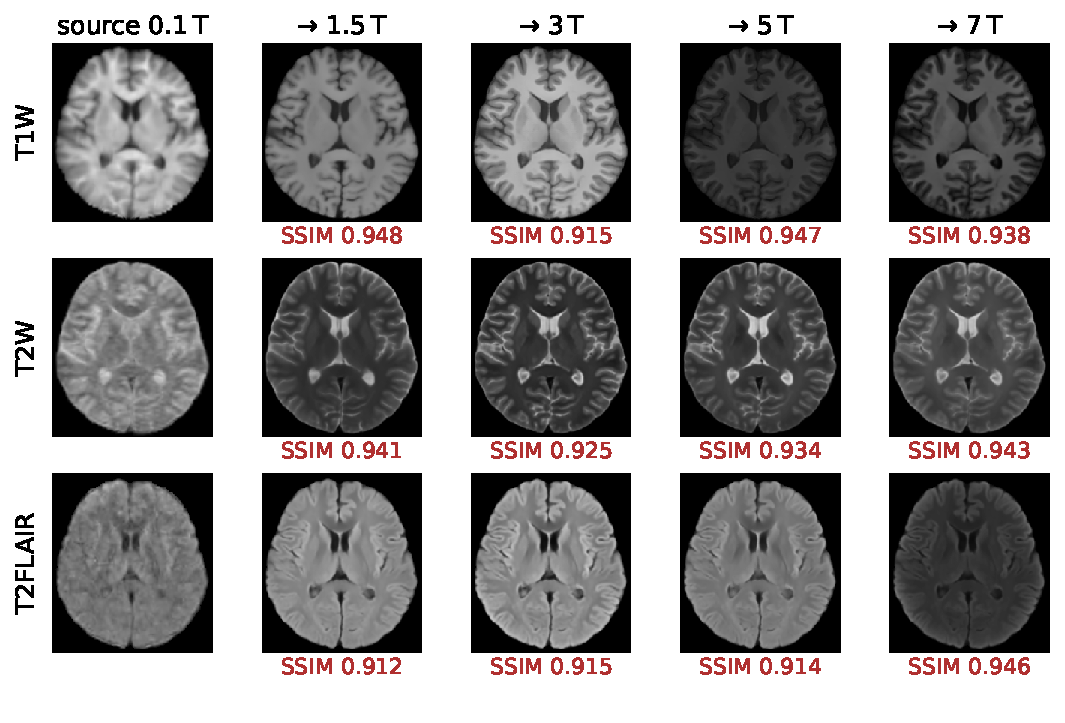
\includegraphics[height=0.76\textheight]{figures/showcase/grid_up_3.pdf}}%
  \only<4>{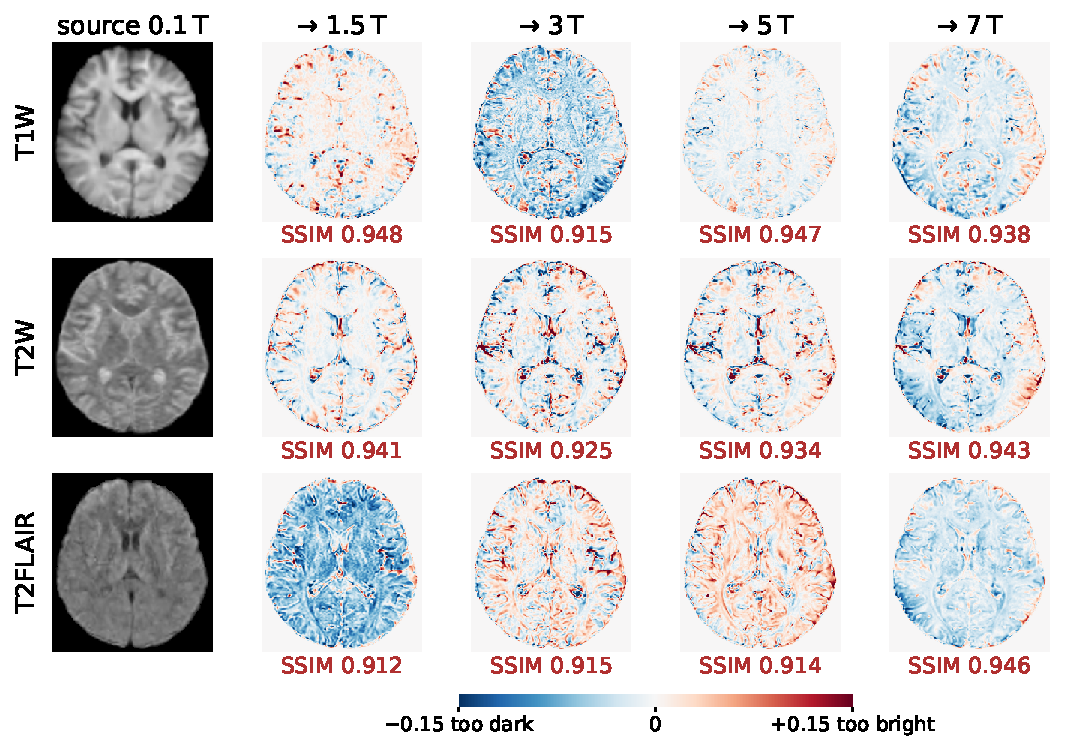
\includegraphics[height=0.76\textheight]{figures/showcase/grid_up_res.pdf}}

  \vspace{0.5mm}
  \only<1-3>{\gloss{From 0.1\,T to every higher field; slab SSIM under each prediction. Subject 0006, in-sample.}}%
  \only<4>{\gloss{Prediction minus target; blue too dark, red too bright. Subject 0006, in-sample.}}
\end{frame}

% --------------------------------------------------- 15. qualitative, to a lower field
\begin{frame}{Predictions to a lower field}
  \ph{TBD}
  \parttag{III \quad METHOD}
  \centering
  \only<1>{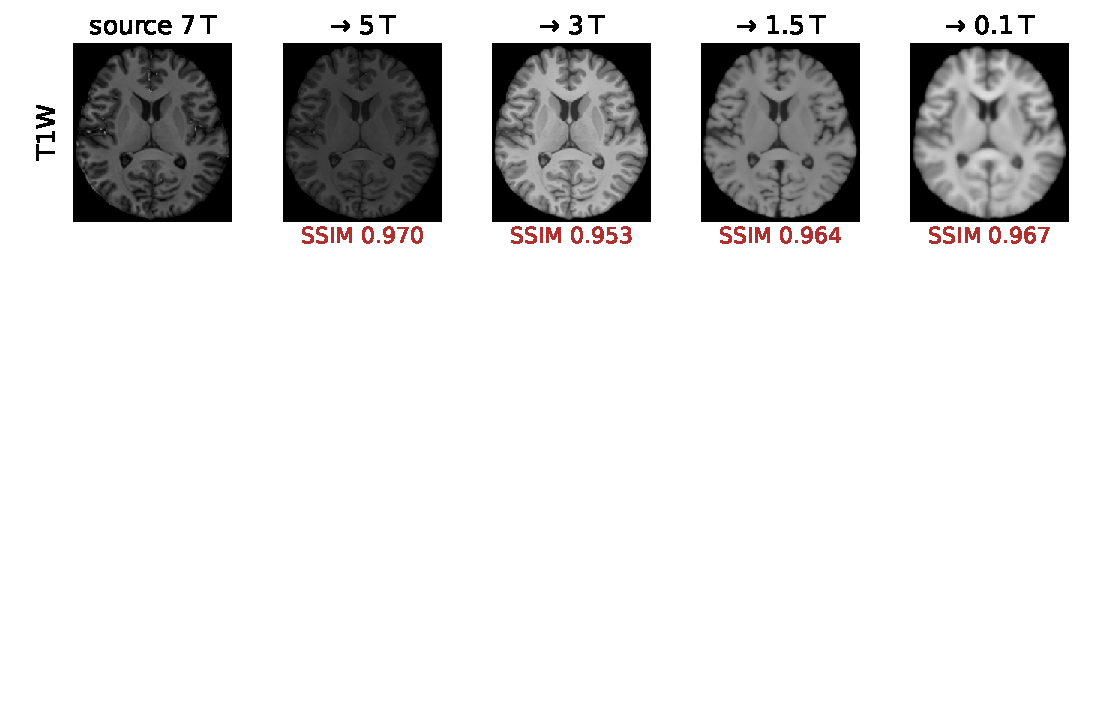
\includegraphics[height=0.76\textheight]{figures/showcase/grid_down_1.pdf}}%
  \only<2>{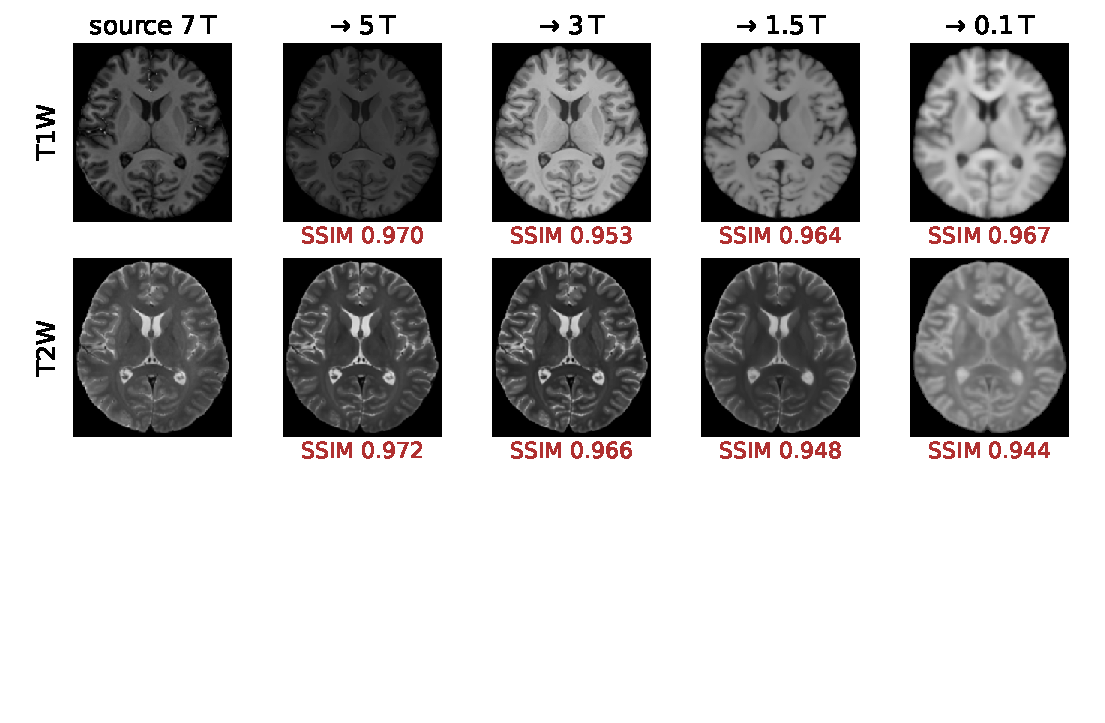
\includegraphics[height=0.76\textheight]{figures/showcase/grid_down_2.pdf}}%
  \only<3>{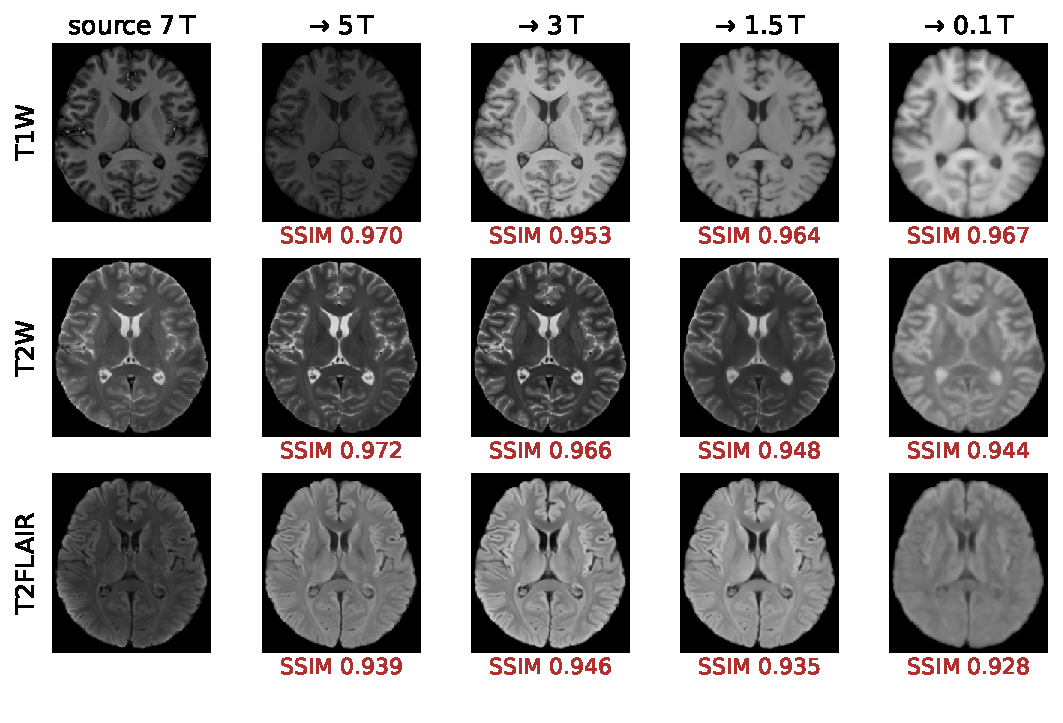
\includegraphics[height=0.76\textheight]{figures/showcase/grid_down_3.pdf}}%
  \only<4>{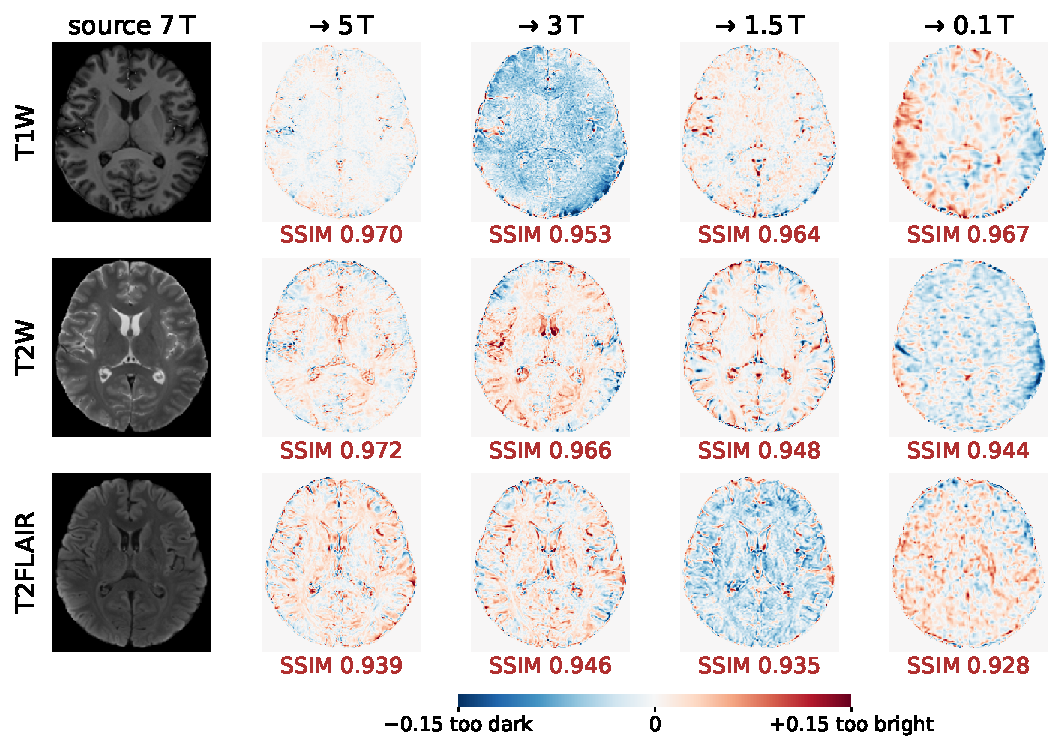
\includegraphics[height=0.76\textheight]{figures/showcase/grid_down_res.pdf}}

  \vspace{0.5mm}
  \only<1-3>{\gloss{From 7\,T to every lower field; slab SSIM under each prediction. Subject 0006, in-sample.}}%
  \only<4>{\gloss{Prediction minus target; blue too dark, red too bright. Subject 0006, in-sample.}}
\end{frame}

% ====================================================== IV. ERROR SPECTRUM
% -------------------------------------------------- 16. error spectrum
\begin{frame}{Error spectrum of the final model}
  \ph{TBD}
  \parttag{IV \quad ERROR SPECTRUM}
  \centering
  \only<1-3>{\maskedfigure{0.96\textwidth}{spectral/fig_error_rapsd_by_field.pdf}{%
    \fill<1>[dim] (0.33,0) rectangle (1.01,1.01);
    \fill<1-2>[dim] (0.66,0) rectangle (1.01,1.01);}}%
  \only<4>{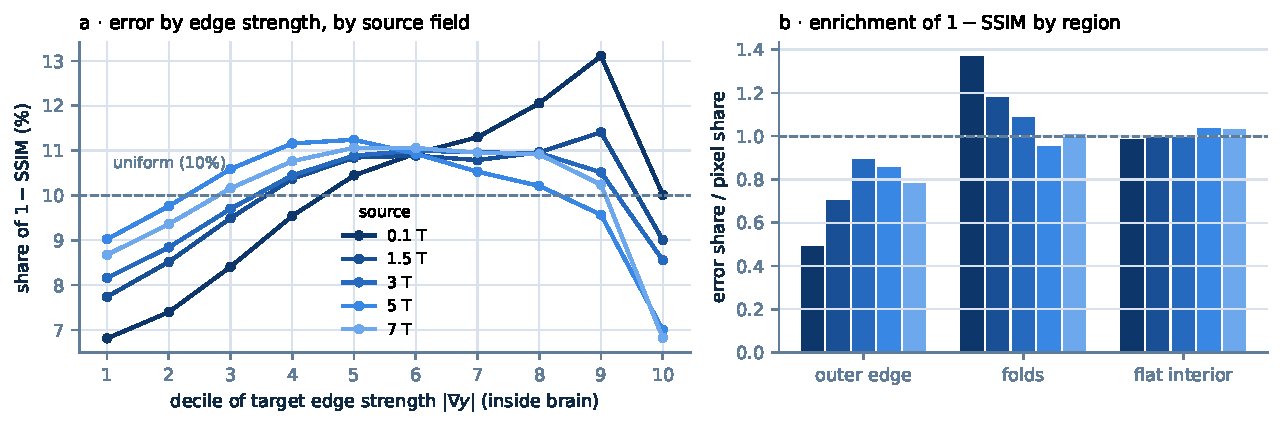
\includegraphics[width=0.80\textwidth]{spectral/fig_error_by_edge.pdf}}

  \vspace{3mm}
  \only<1>{\gloss{\textbf{a.} Error power over target power rises with frequency at every source
  field and passes 1 above $\sim$0.3 cycles/pixel.}}%
  \only<2>{\gloss{\textbf{b.} Cumulative error: 47\% of the error energy is below 0.05
  cycles/pixel and 45\% in 0.05--0.2. For the copy baseline, 97\% is below 0.05.}}%
  \only<3>{\gloss{\textbf{c.} Away from and toward high field, the curves overlap within 10\%
  in every band: the direction does not change the error spectrum.}}%
  \only<4>{\gloss{Squared error: 35\% of it is on fold pixels, 18\% of the brain.
  $1-\mathrm{SSIM}$ on folds: 1.14$\times$ their pixel share.}}
\end{frame}

% --------------------------------------------- 17. smoothness
\begin{frame}{Prediction smoothness}
  \ph{TBD}
  \parttag{IV \quad ERROR SPECTRUM}
  \centering
  \maskedfigure{0.96\textwidth}{spectral/fig_error_smoothness.pdf}{%
    \fill<1>[dim] (0.343,0) rectangle (1.01,1.01);
    \fill<1-2>[dim] (0.664,0) rectangle (1.01,1.01);}

  \vspace{2mm}
  \only<1>{\gloss{\textbf{a.} Prediction power is below target power in every band: 0.72 of it
  at 0.1--0.2 cycles/pixel.}}%
  \only<2>{\gloss{\textbf{b.} Too smooth for every target field up to 0.2 cycles/pixel; above
  that, 0.1\,T targets are noise.}}%
  \only<3>{\gloss{\textbf{c.} SSIM loses most on structure (0.076 on folds, 0.073 in the flat
  interior), then contrast; luminance only at the outer edge.}}%
  \only<4>{\gloss{Post-hoc sharpening, 17 settings: selection on held-out subjects picks no
  sharpening; the best setting per transition gains +0.00004.}}
\end{frame}

% --------------------------------------------- 18. spectral-profile loss
\begin{frame}{Spectral-profile loss}
  \ph{TBD}
  \parttag{IV \quad ERROR SPECTRUM}
  \centering
  \maskedfigure{0.96\textwidth}{spectral/fig_spectral_loss.pdf}{%
    \fill<1>[dim] (0.333,0) rectangle (1.01,1.01);
    \fill<1-2>[dim] (0.667,0) rectangle (1.01,1.01);}

  \vspace{2mm}
  \only<1>{\gloss{\textbf{a.} $\Delta\alpha$-gated spectral-profile loss, one fine-tune: power at
  0.1--0.2 cycles/pixel rises from 0.743 to 0.882 of the target's.}}%
  \only<2>{\gloss{\textbf{b.} Coherence with the target is unchanged: 0.833 $\to$ 0.822.}}%
  \only<3>{\gloss{\textbf{c.} So the error power rises with it, 0.307 $\to$ 0.339 of the
  target's. SSIM $-0.00118$; 164 of 168 transitions lower.}}
\end{frame}

% ============================================================ V. OTHER METHODS
% ------------------------------------------------------------ 19. other backbones
\begin{frame}{Other backbones}
  \ph{TBD}
  \parttag{V \quad OTHER METHODS}
  \centering
  \vspace{2mm}
  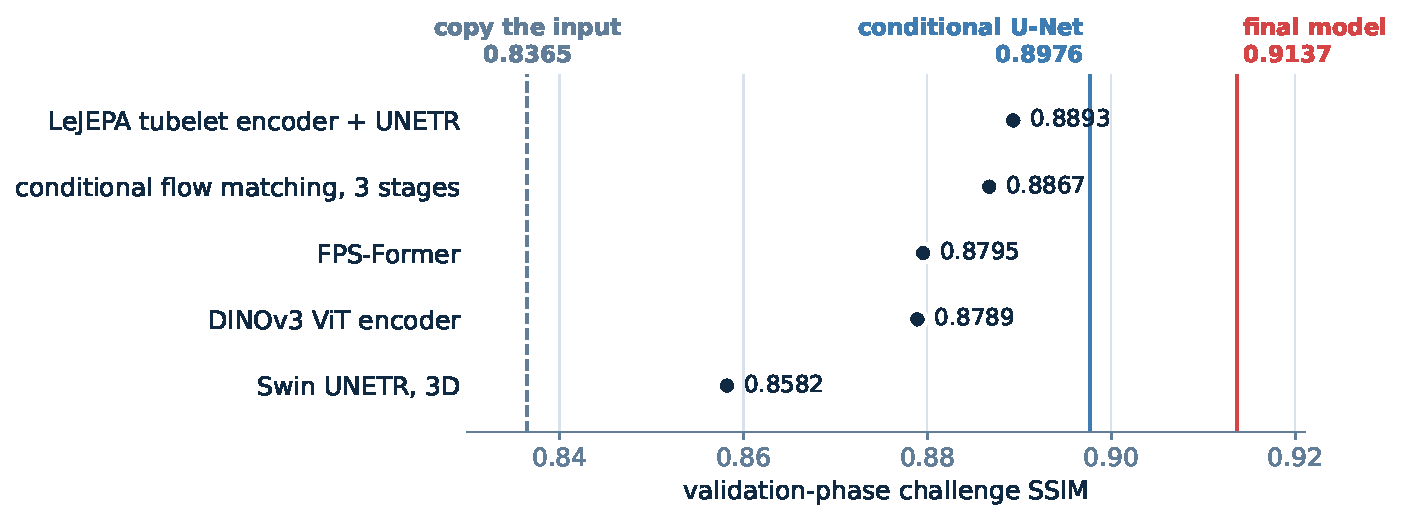
\includegraphics[width=0.94\textwidth]{figures/showcase/other_backbones.pdf}

  \vspace{2mm}
  \gloss{Validation-phase challenge SSIM. All five score below the conditional U-Net.}
\end{frame}

% ------------------------------------------------------------ 20. other changes
\begin{frame}{Other changes}
  \ph{TBD}
  \parttag{V \quad OTHER METHODS}
  \centering
  \only<1>{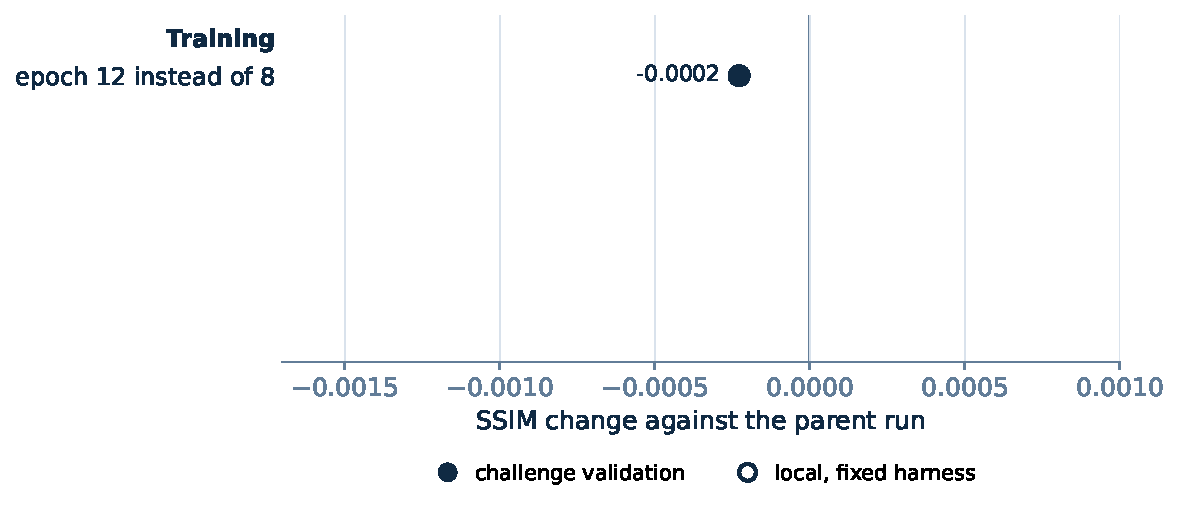
\includegraphics[width=0.84\textwidth]{figures/showcase/other_changes_1.pdf}}%
  \only<2>{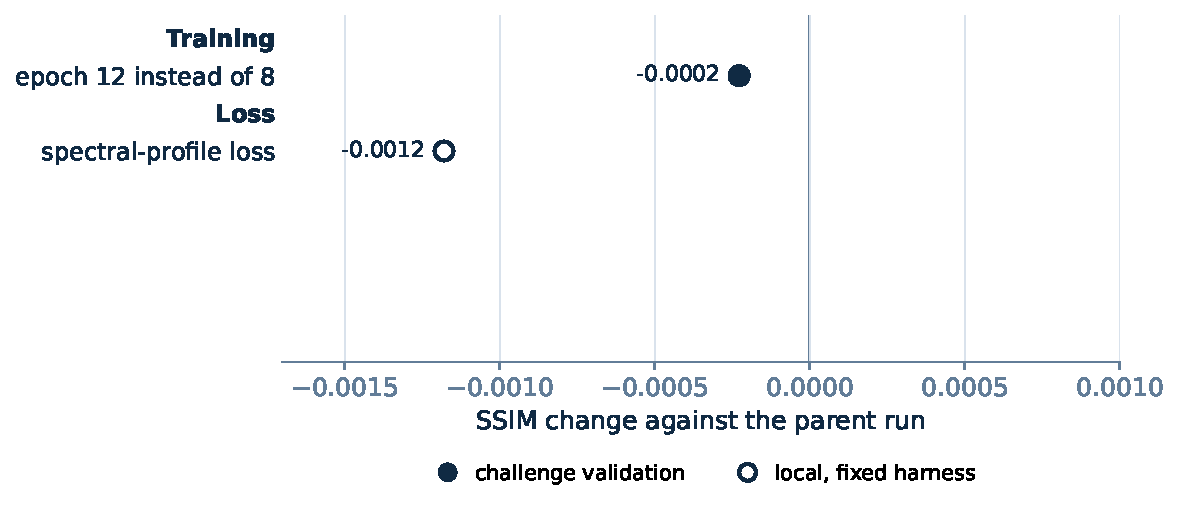
\includegraphics[width=0.84\textwidth]{figures/showcase/other_changes_2.pdf}}%
  \only<3>{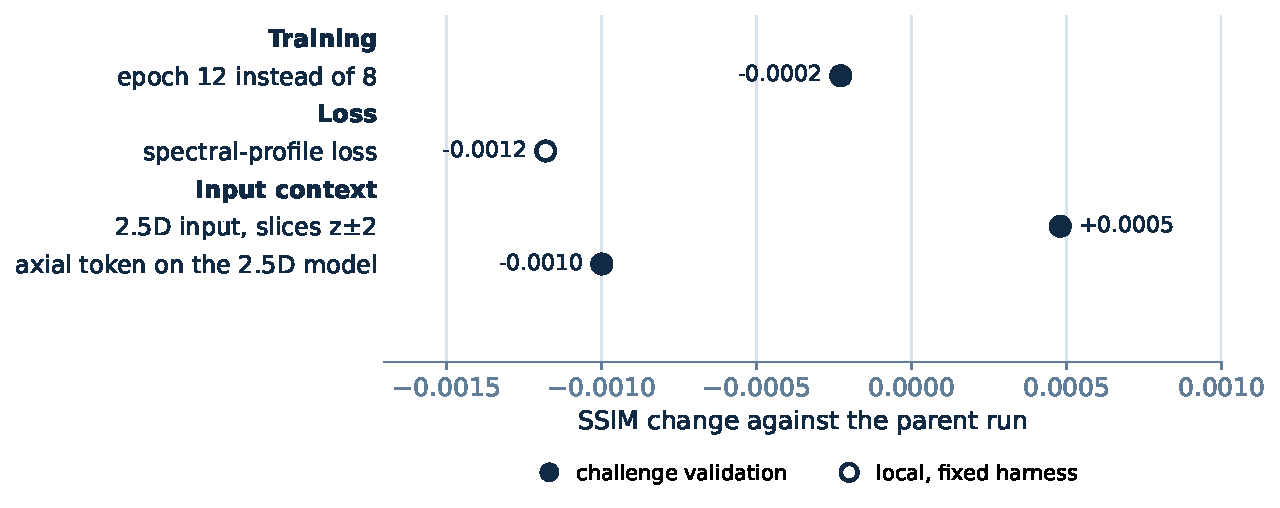
\includegraphics[width=0.84\textwidth]{figures/showcase/other_changes_3.pdf}}%
  \only<4>{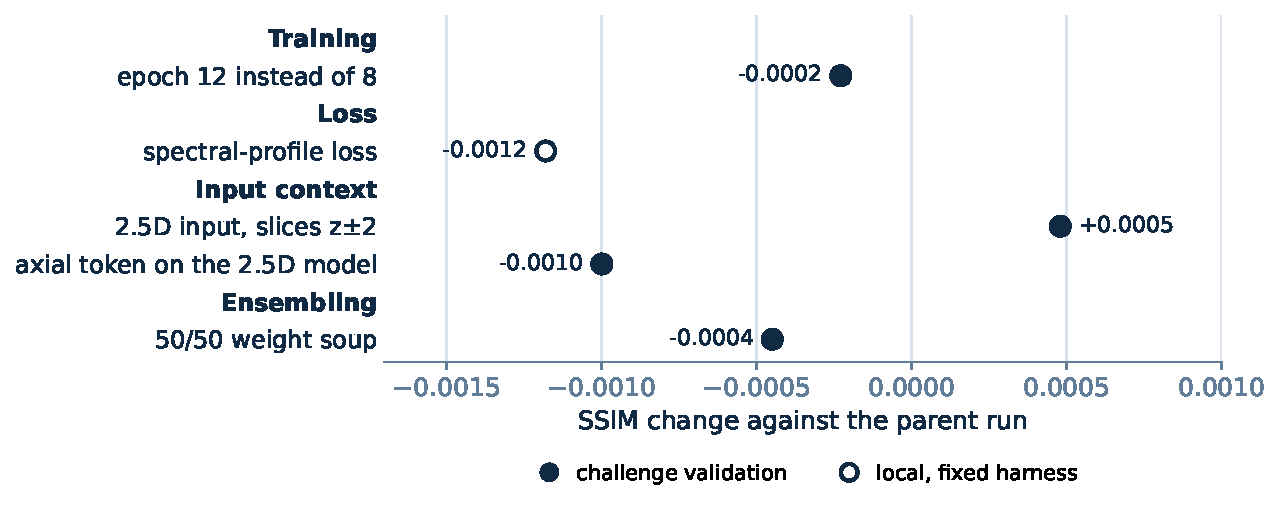
\includegraphics[width=0.84\textwidth]{figures/showcase/other_changes_4.pdf}}

  \vspace{1mm}
  \only<1>{\gloss{Training: epoch 12 instead of 8, preferred by every local check, $-0.0002$ on the
  leaderboard.}}%
  \only<2>{\gloss{Loss: the spectral-profile loss, $-0.0012$ locally; 164 of 168 transitions
  lower.}}%
  \only<3>{\gloss{Input context: 2.5D alone $+0.0005$; the axial token on top of it $-0.0010$.}}%
  \only<4>{\gloss{Ensembling: a 50/50 soup with a sibling run, $-0.0004$.}}
  \srcline{Change against the parent run. Local: fixed harness, in-sample. Full tree:
  \texttt{reports/decision\_tree.pdf}.}
\end{frame}

% -------------------------------------------------- 21. other routes
\begin{frame}{Other routes}
  \ph{TBD}
  \parttag{V \quad OTHER METHODS}
  \centering
  \vspace{4mm}
  {\small
  \begin{tabular}{>{\raggedright\arraybackslash}p{3.2cm}>{\raggedright\arraybackslash}p{4.4cm}>{\raggedright\arraybackslash}p{5.0cm}}
    \toprule
    Constraint & Route & Outcome \\
    \midrule
    \onslide<1->{Unpaired data, 1{,}939 volumes} & \onslide<1->{masked image modelling, whole U-Net}
      & \onslide<1->{kept: $+0.0103$ SSIM} \\[1mm]
    & \onslide<2->{tubelet ViT encoder, LeJEPA} & \onslide<2->{dropped: 0.8590 SSIM} \\[1mm]
    \onslide<3->{Paired data, 3 volunteers} & \onslide<3->{synthetic pairs from degraded 7\,T}
      & \onslide<3->{dropped before training: the 0.1\,T error is information-limited} \\[1mm]
    \onslide<4->{Frequency bands} & \onslide<4->{FPS-Former, band split in attention}
      & \onslide<4->{dropped: 0.8795 SSIM, LPIPS 0.149} \\
    \bottomrule
  \end{tabular}}
\end{frame}

% =========================================================== VI. RESULTS
% ------------------------------------------------------------ 22. final ranking
\begin{frame}{Final test ranking, Task 3}
  \ph{TBD}
  \parttag{VI \quad RESULTS}
  \centering
  \vspace{1mm}
  \only<1>{\finaltable{}{}}%
  \only<2>{\finaltable{\rowcolor{baseline!70}}{}}%
  \only<3>{\finaltable{\rowcolor{baseline!70}}{\textbf}}

  \vspace{3mm}
  \only<1>{\gloss{Test phase: 20 volunteers, Docker submission. Top 9 of 25 teams, ordered by
  SSIM.}}%
  \only<2>{\gloss{Mean rank: 6th, tied.}}%
  \only<3>{\gloss{SSIM is the main metric; we are 4th on it.}}
\end{frame}

% ------------------------------------------------------------ 23. trade-off
\begin{frame}{The trade-off}
  \ph{TBD}
  \parttag{VI \quad RESULTS}
  \begin{columns}[t,onlytextwidth]
  \begin{column}{0.49\textwidth}
    \centering
    {\footnotesize\bfseries validation: our submissions}\par\vspace{1mm}
    \only<1>{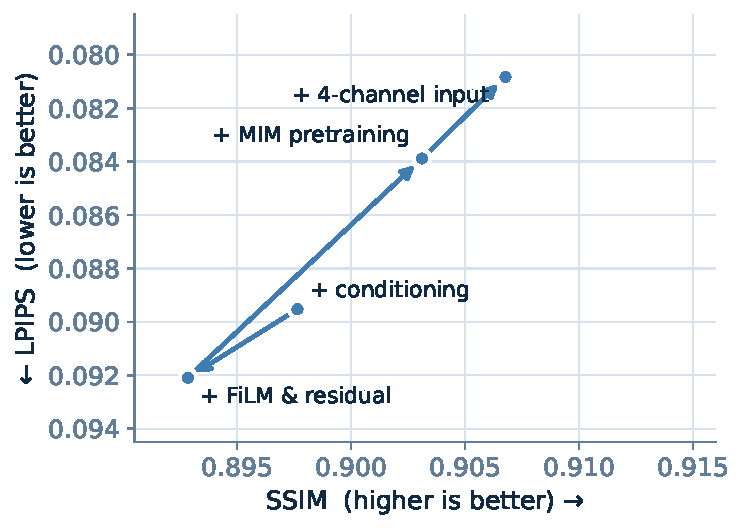
\includegraphics[width=\linewidth]{figures/showcase/trade_ladder_1.pdf}}%
    \only<2->{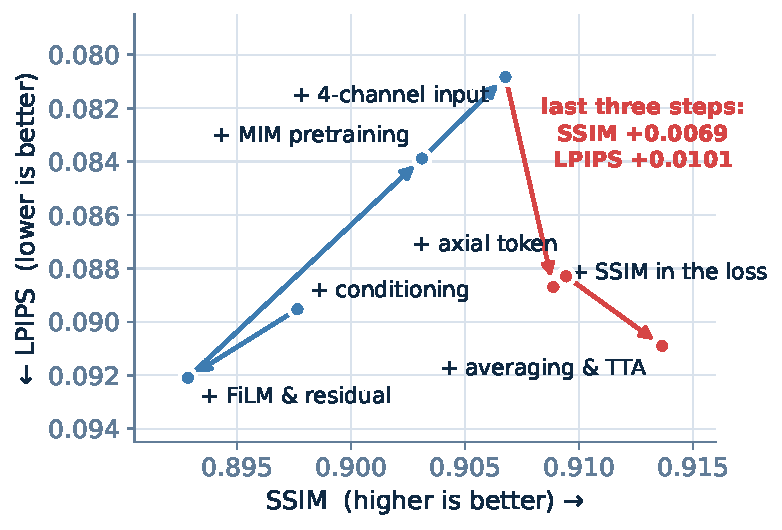
\includegraphics[width=\linewidth]{figures/showcase/trade_ladder_2.pdf}}
  \end{column}
  \begin{column}{0.49\textwidth}
    \centering
    \onslide<3->{{\footnotesize\bfseries test: the top 9}\par\vspace{1mm}}
    \only<1-2>{\phantom{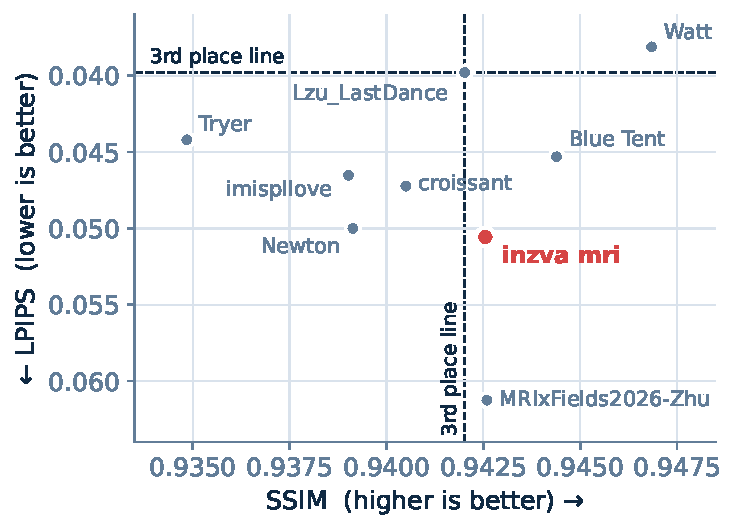
\includegraphics[width=\linewidth]{figures/showcase/trade_final.pdf}}}%
    \only<3>{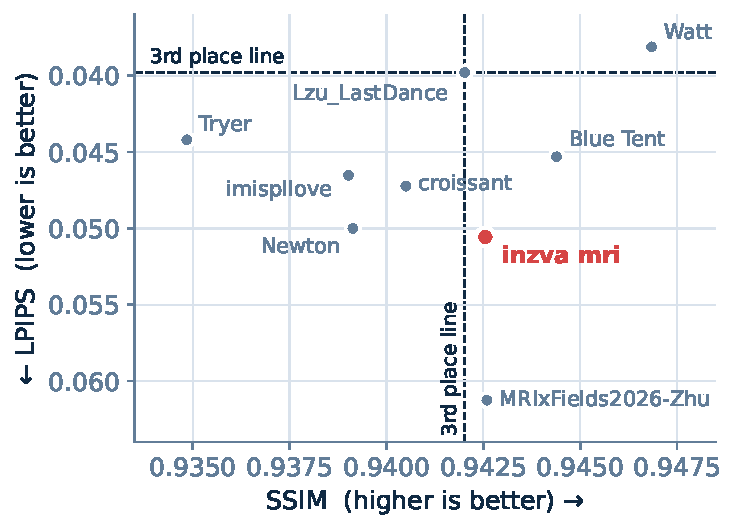
\includegraphics[width=\linewidth]{figures/showcase/trade_final.pdf}}
  \end{column}
  \end{columns}

  \vspace{2mm}
  \only<1>{\gloss{Up to the 4-channel input, SSIM and LPIPS both improved.}}%
  \only<2>{\gloss{The last three steps targeted SSIM, the main metric: SSIM $+0.0069$, LPIPS
  $+0.0101$.}}%
  \only<3>{\gloss{Test phase. Dashed lines: SSIM and LPIPS of the 3rd-placed team.}}
\end{frame}

% ---------------------------------------------------------------- 24. award
\begin{frame}{3rd Place Award, Task 3}
  \ph{TBD}
  \parttag{VI \quad RESULTS}
  \centering
  \vspace{1mm}
  \IfFileExists{figures/showcase/award_certificate.jpg}{%
    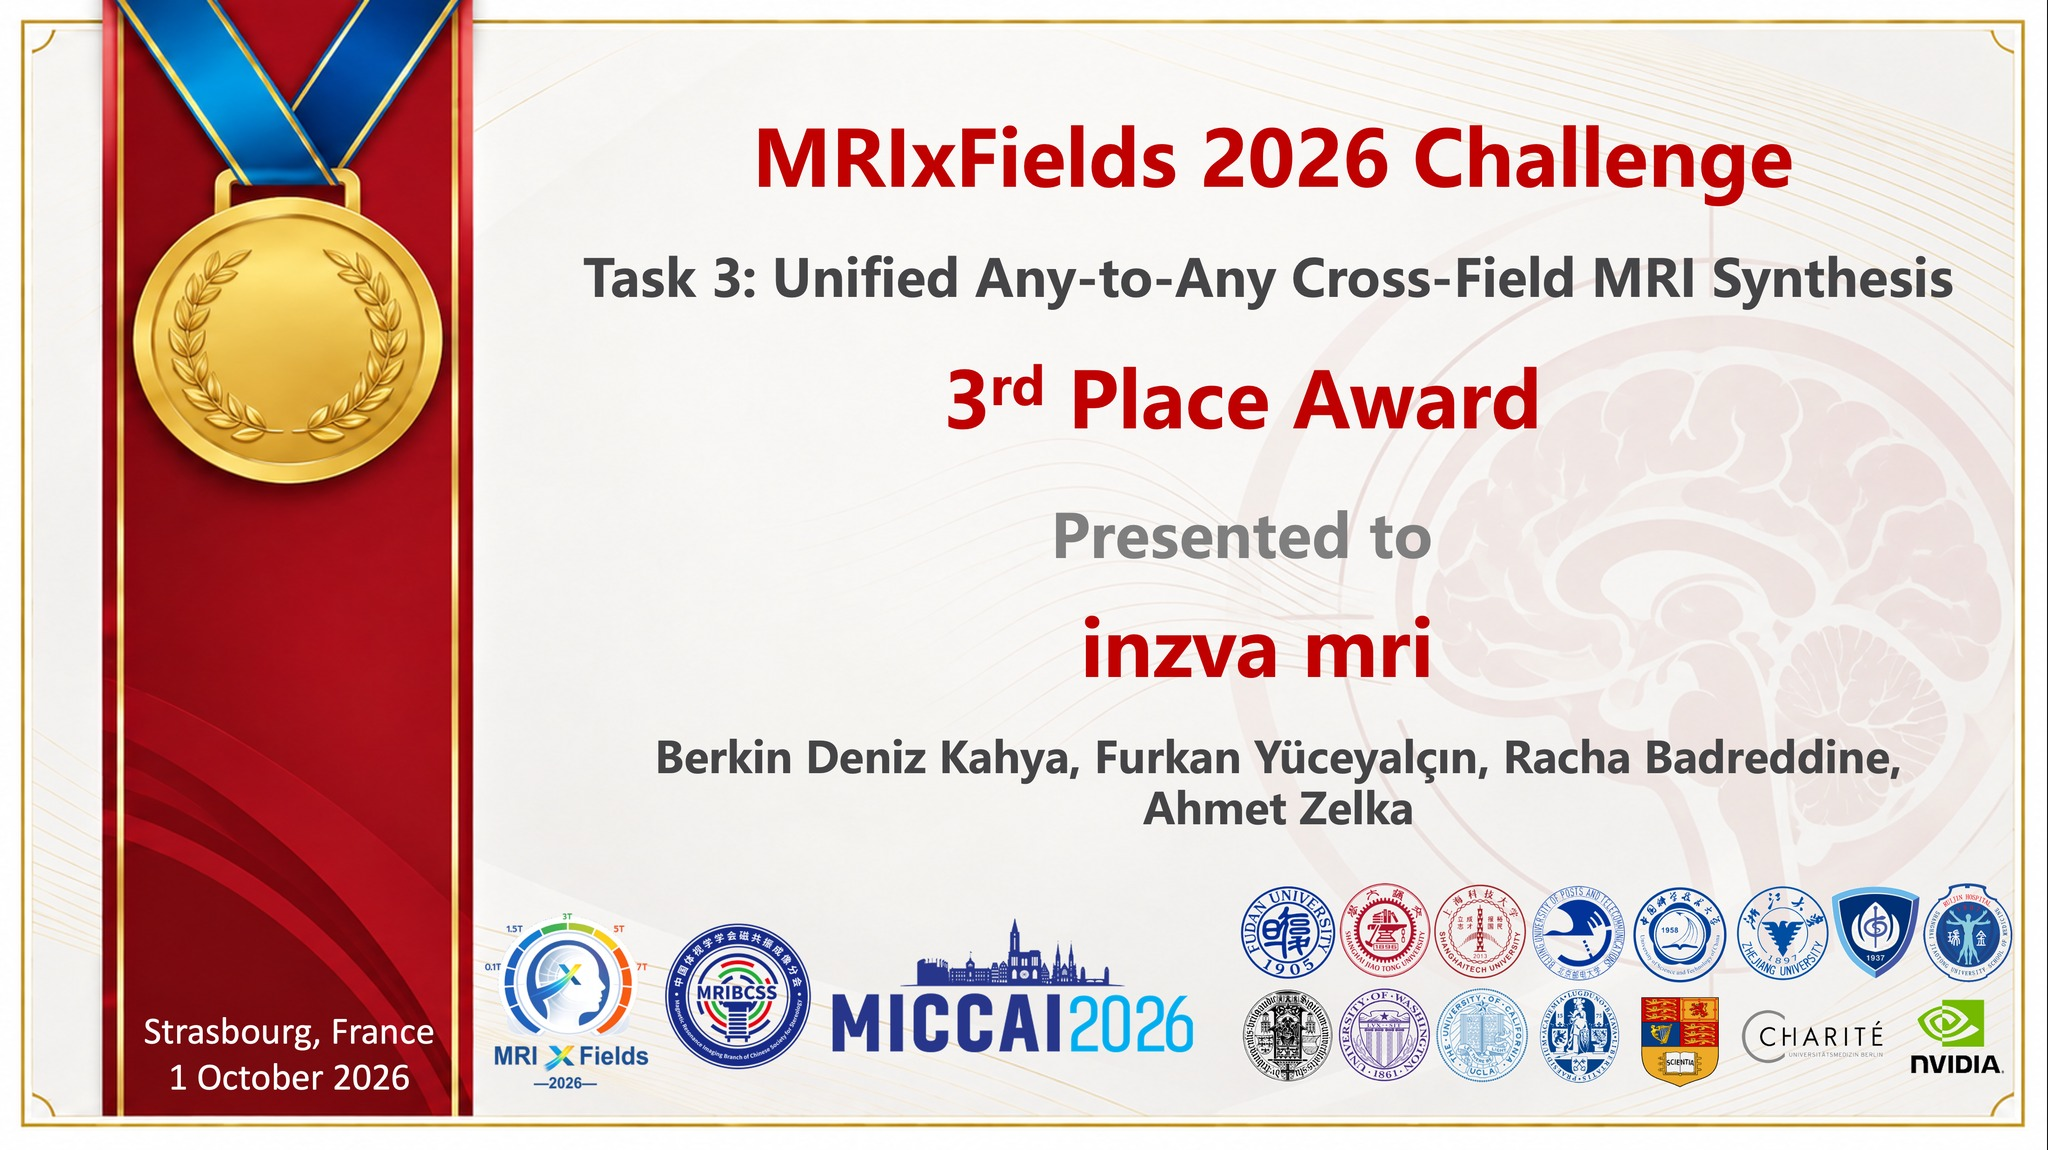
\includegraphics[height=0.70\textheight]{figures/showcase/award_certificate.jpg}}{%
    \placeholder{11cm}{6.2cm}{award certificate}}

  \vspace{2mm}
  \gloss{MRIxFields 2026, MICCAI 2026, Strasbourg, 1 October 2026.}
\end{frame}

% ---------------------------------------------------------------- 25. preprint
\begin{frame}{Preprint}
  \ph{TBD}
  \parttag{VI \quad RESULTS}
  \centering
  \vspace{1mm}
  % first page of the preprint goes here:
  % \includegraphics[height=0.80\textheight]{figures/showcase/preprint_page1.pdf}
  \placeholder{5.2cm}{6.6cm}{first page of the preprint\\(draft in preparation)}
\end{frame}

% ---------------------------------------------------------------- 26. takeaway
\begin{frame}{Takeaway}
  \ph{TBD}
  \parttag{VI \quad RESULTS}
  \centering
  \vspace{12mm}
  {\renewcommand{\arraystretch}{2.1}
  \begin{tabular}{r@{\hspace{7mm}}l}
    \onslide<1->{\Large\textbf{$+$0.0278}} & \onslide<1->{conditioning on the source and target field} \\
    \onslide<2->{\Large\textbf{$+$0.0103}} & \onslide<2->{MIM pretraining on 1{,}939 unpaired volumes} \\
    \onslide<3->{\Large\textbf{none}} & \onslide<3->{from larger backbones, loss reweighting, sharpening,
      a spectral loss} \\
    \onslide<4->{\Large\textbf{$<$0.001}} & \onslide<4->{local scores cannot rank; the leaderboard can} \\
  \end{tabular}}
  \srcline{Validation-phase challenge SSIM.}
\end{frame}

% =========================================================== VII. FUTURE WORK
% ---------------------------------------------------------------- 27. fastMRI data
\begin{frame}{fastMRI}
  \ph{TBD}
  \parttag{VII \quad FUTURE WORK}
  \centering
  \vspace{5mm}
  {\small\renewcommand{\arraystretch}{1.7}
  \begin{tabular}{lll}
    \toprule
    & MRIxFields 2026 & fastMRI brain \\
    \midrule
    \onslide<1->{volumes} & \onslide<1->{1{,}939 unpaired; 3 paired volunteers} & \onslide<1->{6{,}970} \\
    \onslide<2->{field strength} & \onslide<2->{0.1, \textbf{1.5}, \textbf{3}, 5, 7\,T}
      & \onslide<2->{\textbf{1.5}, \textbf{3}\,T; 11 magnets, 5 sites} \\
    \onslide<3->{contrasts} & \onslide<3->{\textbf{T1W}, \textbf{T2W}, \textbf{T2FLAIR}}
      & \onslide<3->{\textbf{T1}, T1-post, \textbf{T2}, \textbf{FLAIR}} \\
    \onslide<4->{data} & \onslide<4->{magnitude images, co-registered}
      & \onslide<4->{raw multi-coil k-space} \\
    \onslide<5->{task} & \onslide<5->{image $\to$ same subject, another field}
      & \onslide<5->{undersampled k-space $\to$ image} \\
    \bottomrule
  \end{tabular}}

  \vspace{3mm}
  \onslide<2->{\gloss{Bold: shared by both.}}
  \srcline{Zbontar et al., \emph{fastMRI: an open dataset and benchmarks for accelerated MRI},
  arXiv:1811.08839.}
\end{frame}

% ---------------------------------------------------------------- 28. k-space
\begin{frame}{fastMRI: reconstruction}
  \ph{TBD}
  \parttag{VII \quad FUTURE WORK}
  \centering
  \vspace{4mm}
  \only<1>{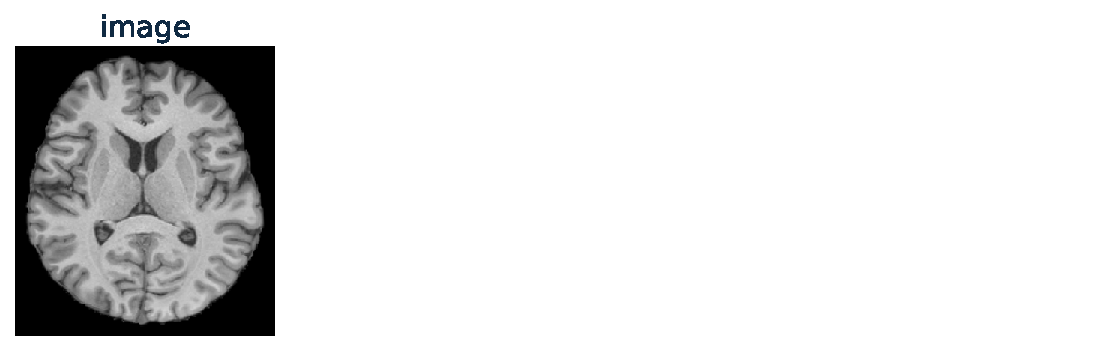
\includegraphics[width=0.92\textwidth]{figures/showcase/kspace_1.pdf}}%
  \only<2>{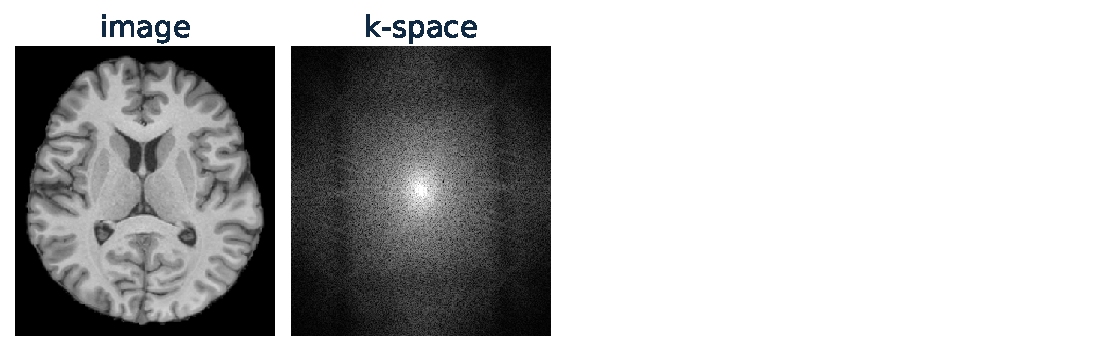
\includegraphics[width=0.92\textwidth]{figures/showcase/kspace_2.pdf}}%
  \only<3>{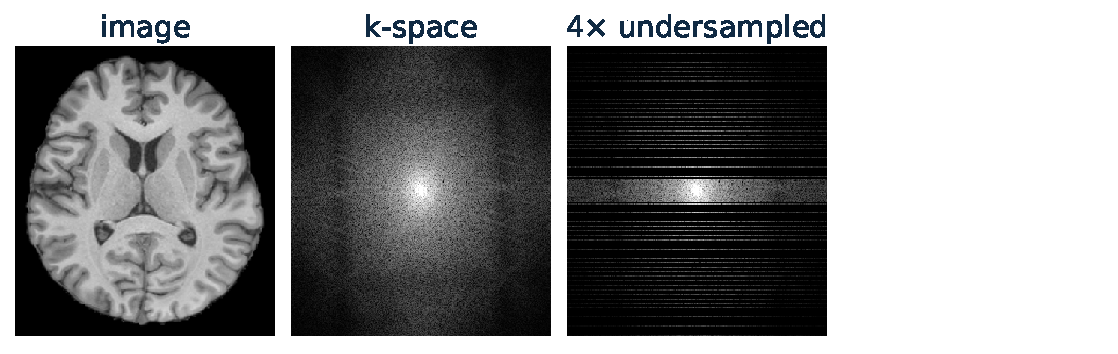
\includegraphics[width=0.92\textwidth]{figures/showcase/kspace_3.pdf}}%
  \only<4>{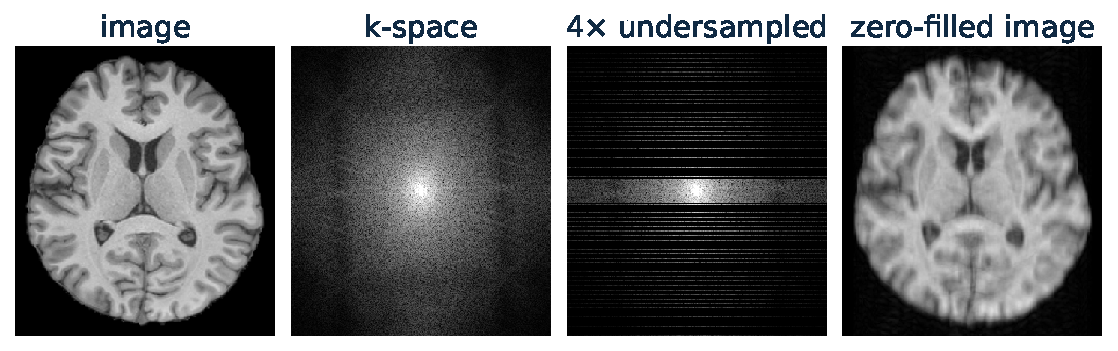
\includegraphics[width=0.92\textwidth]{figures/showcase/kspace_4.pdf}}

  \vspace{3mm}
  \only<1>{\gloss{A 3\,T T1W slice.}}%
  \only<2>{\gloss{The scanner measures k-space, the 2D Fourier transform of the image: the centre
  holds coarse contrast, the outside fine detail.}}%
  \only<3>{\gloss{A 4$\times$ faster scan measures a quarter of the lines: the centre 8\%, the rest
  evenly spaced.}}%
  \only<4>{\gloss{Missing lines set to zero: blur and aliasing. The fastMRI task is to fill them
  in.}}
  \srcline{Simulated from an MRIxFields 3\,T image, subject 0006; fastMRI provides the measured
  k-space.}
\end{frame}

% ---------------------------------------------------------------- 29. future work
\begin{frame}{Future work}
  \ph{TBD}
  \parttag{VII \quad FUTURE WORK}
  \vspace{14mm}
  \begin{itemize}\setlength{\itemsep}{7mm}\large
    \item<1-> Spectral slopes per field strength and contrast, on 6{,}970 volumes
    \item<2-> Coherence per frequency: detail recovered or detail invented
    \item<3-> Noise floor first, then compare models
  \end{itemize}
\end{frame}

% ---------------------------------------------------------------- 30. thank you
{\setbeamertemplate{background}{}
\begin{frame}[plain,noframenumbering]
  \ph{TBD}
  \vfill
  \centering
  {\Large\bfseries Thank you}\\[2mm]
  {\large Questions?}\\[6mm]
  \qrcode[height=2.6cm]{https://github.com/denizberkin/mrixfields-analysis}\\[2.5mm]
  {\footnotesize\texttt{github.com/denizberkin/mrixfields-analysis}}\\[5mm]
  \logoslot{itu_logo_siyah}{\.ITU}{9mm}\hspace{14mm}%
  \raisebox{1.7mm}{\logoslot{inzva_logo_dark}{inzva}{5.5mm}}
  \vfill
\end{frame}
}

% ===================================================================== BACKUP
\appendix

\begin{frame}{Backup: image spectra}
  \ph{TBD}
  \centering
  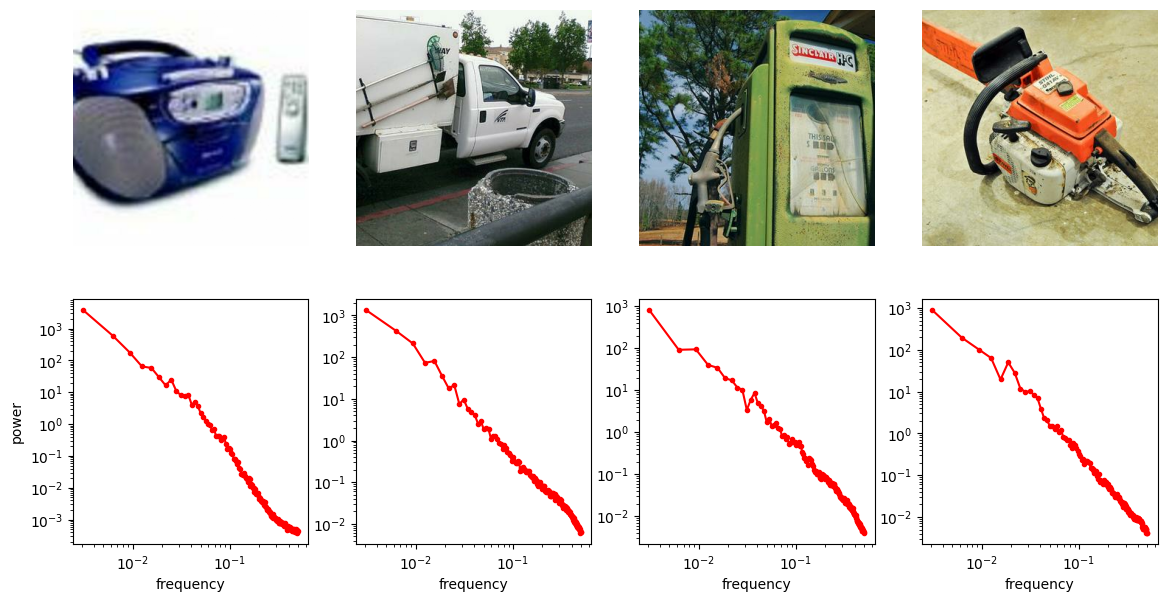
\includegraphics[height=0.56\textheight]{spectral/dieleman/cell21.png}

  \vspace{0.5em}
  \gloss{Average each image's Fourier magnitude over all directions: one power--frequency curve
  per image (RAPSD, radially averaged power spectral density). Natural images follow
  $P(f)\propto f^{-\alpha}$ with $\alpha\approx2$.}
  \srcline{Dieleman, \emph{Diffusion is spectral autoregression} (2024).}
\end{frame}

\begin{frame}{Backup: noise and fine detail}
  \ph{TBD}
  \centering
  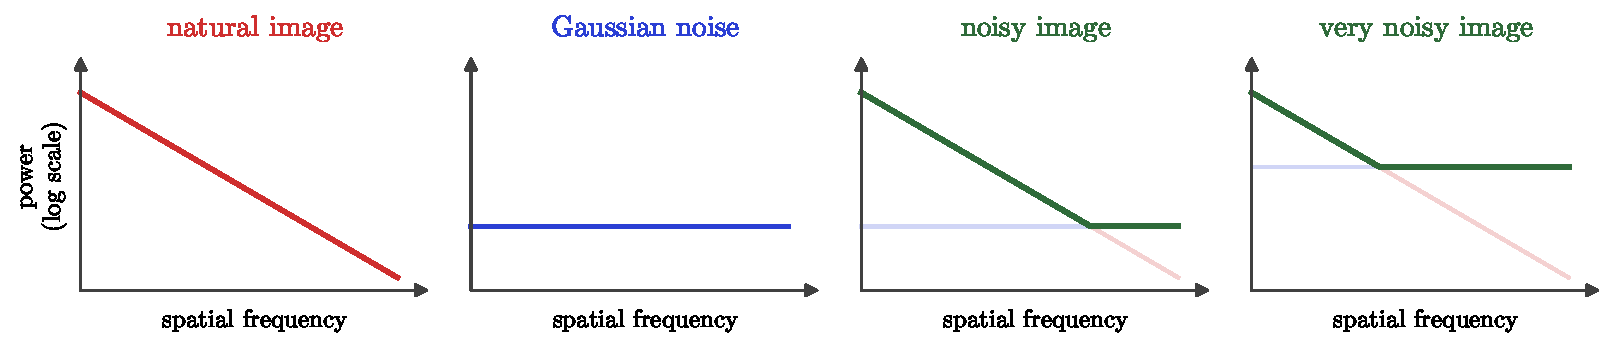
\includegraphics[width=\textwidth]{spectral/fig_noise_schematic.pdf}

  \vspace{0.8em}
  \gloss{Image (red), Gaussian noise (blue), noisy image (green). Noise is flat in frequency,
  so it covers the weak high-frequency end first.}
  \srcline{Schematic redrawn after Dieleman (2024).}
\end{frame}

\begin{frame}{Backup: validation-phase submissions}
  \ph{TBD}
  \centering
  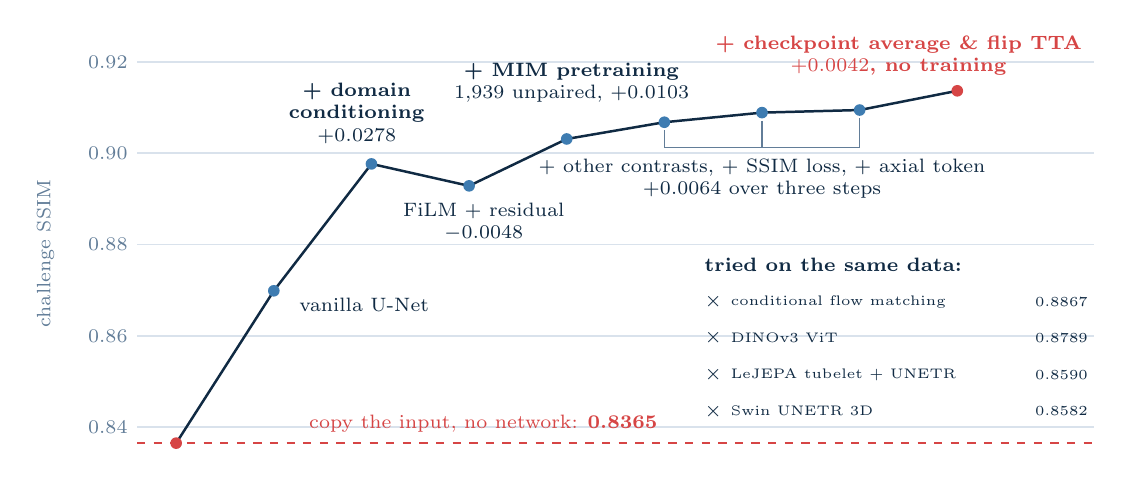
\begin{tikzpicture}[x=1.24cm,y=58cm,font=\scriptsize]
    \foreach \v/\lab in {0.010/0.84,0.030/0.86,0.050/0.88,0.070/0.90,0.090/0.92}{
      \draw[draw=baseline,line width=0.6pt] (-0.4,\v) -- (9.4,\v);
      \node[text=muted,anchor=east,inner sep=1.5pt] at (-0.45,\v) {\lab};}
    \node[text=muted,rotate=90,anchor=south] at (-1.15,0.048) {challenge SSIM};
    \draw[accent,dashed,line width=0.7pt] (-0.4,0.006497) -- (9.4,0.006497);
    \node[text=accent,anchor=west,inner sep=2pt] at (1.3,0.0108)
      {copy the input, no network: \textbf{0.8365}};
    \draw[ink,line width=0.9pt]
      (0,0.006497) -- (1,0.039856) -- (2,0.067646) -- (3,0.062839) --
      (4,0.073110) -- (5,0.076773) -- (6,0.078873) -- (7,0.079433) -- (8,0.083652);
    \foreach \x/\y in {1/0.039856, 2/0.067646, 3/0.062839, 4/0.073110,
                       5/0.076773, 6/0.078873, 7/0.079433}{
      \fill[cond] (\x,\y) circle (2.1pt);}
    \fill[accent] (0,0.006497) circle (2.1pt);
    \fill[accent] (8,0.083652) circle (2.1pt);
    \node[text=ink,anchor=west,inner sep=2pt] at (1.2,0.0368) {vanilla U-Net};
    \node[text=ink,anchor=south,align=center,inner sep=3pt] at (1.85,0.0702)
      {\textbf{+ domain}\\\textbf{conditioning}\\$+0.0278$};
    \node[text=ink,anchor=north,align=center,inner sep=2.5pt] at (3.15,0.0607)
      {FiLM $+$ residual\\$-0.0048$};
    \node[text=ink,anchor=south,align=center,inner sep=3pt] at (4.05,0.0792)
      {\textbf{+ MIM pretraining}\\1{,}939 unpaired, $+0.0103$};
    \foreach \x/\y in {5/0.076773, 6/0.078873, 7/0.079433}{
      \draw[draw=muted,line width=0.4pt] (\x,{\y-0.0018}) -- (\x,0.0712);}
    \draw[draw=muted,line width=0.4pt] (5,0.0712) -- (7,0.0712);
    \node[text=ink,anchor=north,align=center,inner sep=3pt] at (6,0.0706)
      {+ other contrasts, + SSIM loss, + axial token\\$+0.0064$ over three steps};
    \node[text=accent,anchor=south,align=center,inner sep=3pt] at (7.4,0.0851)
      {\textbf{+ checkpoint average \& flip TTA}\\\textbf{$+0.0042$, no training}};
    \node[text=ink,anchor=west,inner sep=2pt,font=\scriptsize] at (5.35,0.0455)
      {\textbf{tried on the same data:}};
    \foreach \y/\lab/\val in {0.0375/{conditional flow matching}/0.8867,
                              0.0295/{DINOv3 ViT}/0.8789,
                              0.0215/{LeJEPA tubelet + UNETR}/0.8590,
                              0.0135/{Swin UNETR 3D}/0.8582}{
      \node[text=ink] at (5.5,\y) {$\times$};
      \node[text=ink,anchor=west,font=\tiny,inner sep=2pt] at (5.62,\y) {\lab};
      \node[text=ink,anchor=east,font=\tiny,inner sep=2pt] at (9.4,\y) {\val};}
  \end{tikzpicture}
\end{frame}

\begin{frame}{Backup: top teams' methods}
  \ph{TBD}
  \footnotesize
  \begin{tabular}{@{}llp{8.4cm}@{}}
    \toprule
    rank & team & method (workshop paper) \\
    \midrule
    1 & Watt (MSRA) & source-conditioned translation with shared-cycle refinement \\
    2 & Blue Tent (Warwick) & latent bridge matching: Stable Diffusion 2.1 VAE + Marigold U-Net,
      one step, LPIPS weight 0.2 \\
    3 & Lzu\_LastDance (Lanzhou) & FieldMorphUNet, structure-scale decoupling \\
    4 & croissant (NEUROPHET) & paired--synthetic--paired latent diffusion \\
    5 & Newton (Leiden UMC) & conditional flow matching + adversarial refinement \\
    6 & inzva mri (ITU, inzva) & MIM pretraining + conditioning (this talk) \\
    8 & MRIxFields2026-Zhu (UW) & frozen DINOv3 + DPT decoder; FiLM output-stack cascade \\
    \bottomrule
  \end{tabular}

  \vspace{3mm}
  \gloss{From the 22 workshop papers on the challenge's Synapse page; Blue Tent's and Newton's
  are on arXiv (2609.20341, 2609.00960).}
\end{frame}

\end{document}
